\documentclass[aspectratio=169]{beamer}
\setbeamertemplate{navigation symbols}{}
\usepackage{color, amsmath, comment, subfigure}
\usepackage{url}
\usepackage{tikz}

\usepackage{hyperref}
\hypersetup{
    colorlinks=true,
    linkcolor=blue,
    filecolor=magenta,      
    urlcolor=cyan,
}

\newcommand\red[1]{{\color{red}#1}}
\newcommand\bred[1]{{\color{red}\textbf{#1}}}
\newcommand\blue[1]{{\color{blue}#1}}
\newcommand\bblue[1]{{\color{blue}\textbf{#1}}}
\newcommand\green[1]{{\color{olive}#1}}
\newcommand\bgreen[1]{{\color{olive}\textbf{#1}}}
\newcommand\black[1]{{\color{black}#1}}
\newcommand\white[1]{{\color{white}#1}}
\newcommand\E{\text{E}}
\newcommand\V{\text{V}}
\renewcommand\P{\text{P}}


%%%%%%%%%%%%%%%%%%%%%%%%%%
\title[]{Pre-read for Tuesday, November 5:\\Predictability of life trajectories}
\author[]{Matthew J. Salganik}
\institute[]{}
\date[]{COS 597E/SOC 555 Limits to prediction\\Fall 2020, Princeton University}

\begin{document}
%%%%%%%%%%%%%%%%%%%%%%%%%%%
\frame{\titlepage}
%%%%%%%%%%%%%%%%%%%%%%%%%%%
\begin{frame}

\begin{center}

\includegraphics[width=0.65\textwidth]{figures/wikipedia_logo}
\end{center}

\end{frame}
%%%%%%%%%%%%%%%%%%%%%%%%%%%
\begin{frame}

\begin{center}
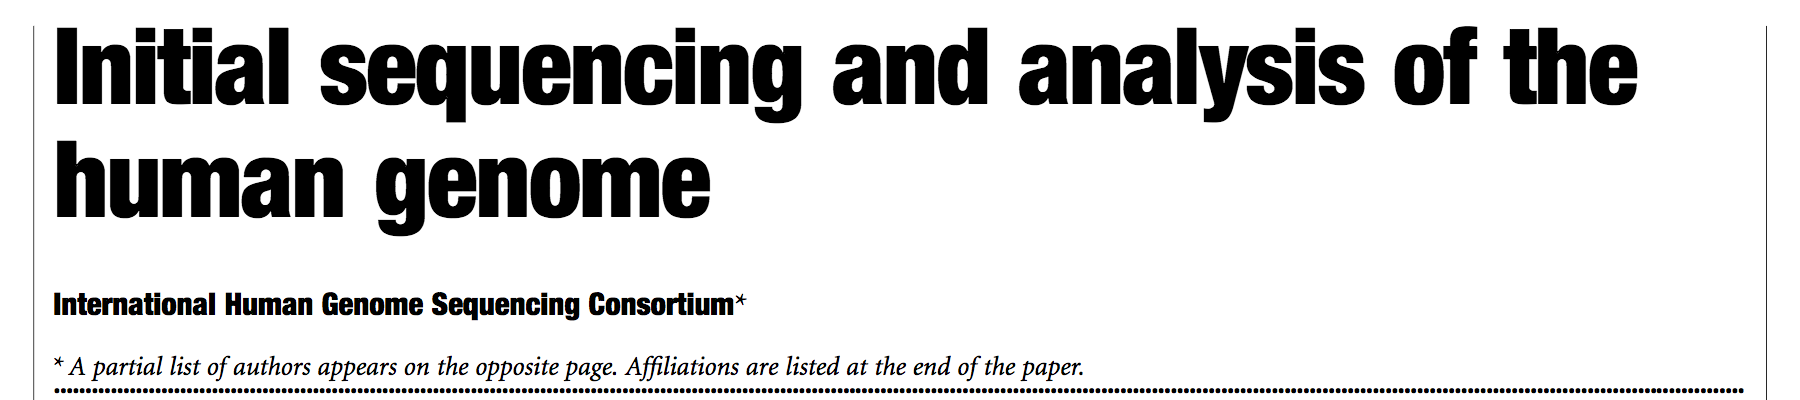
\includegraphics[width=\textwidth]{figures/lander_initial_2001_title}
\end{center}

\vfill
{\tiny \url{http://dx.doi.org/10.1038/35057062}}

\end{frame}
%%%%%%%%%%%%%%%%%%%%%%%%%%
\begin{frame}

\begin{center}
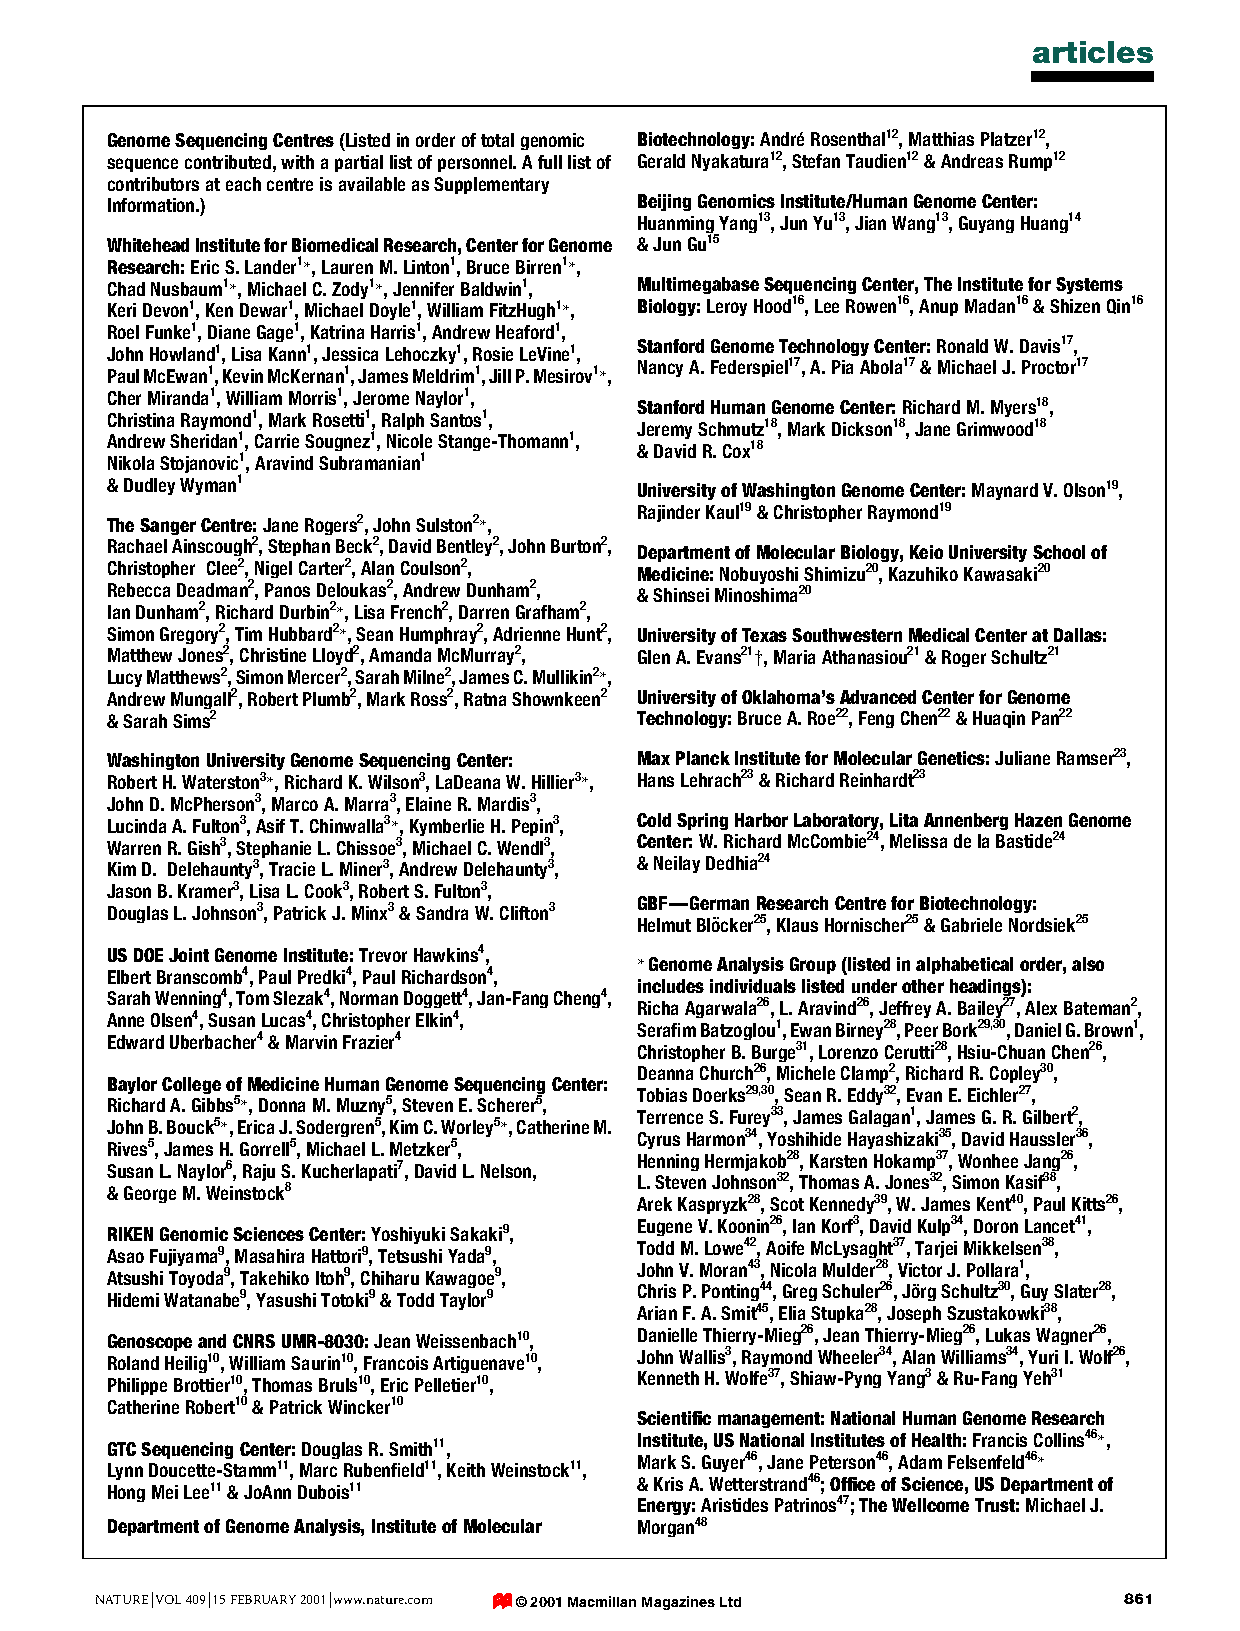
\includegraphics[height=\textheight]{figures/lander_initial_2001_authors}
\end{center}

\end{frame}
%%%%%%%%%%%%%%%%%%%%%%%%%%
\begin{frame}

\begin{center}
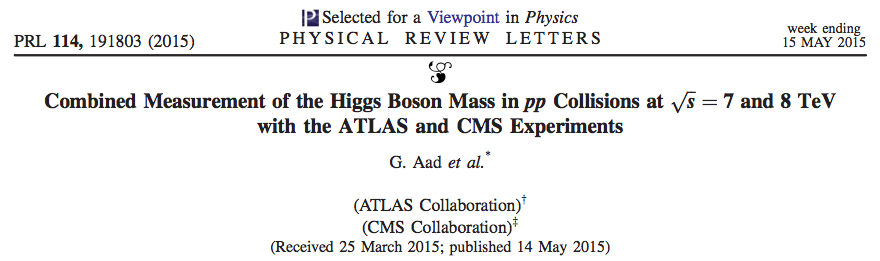
\includegraphics[width=\textwidth]{figures/aad_combined_2015_title}
\end{center}

\vfill
{\tiny \url{https://doi.org/10.1103/PhysRevLett.114.191803}}

\end{frame}
%%%%%%%%%%%%%%%%%%%%%%%%%%
\begin{frame}

\begin{center}
\only<1>{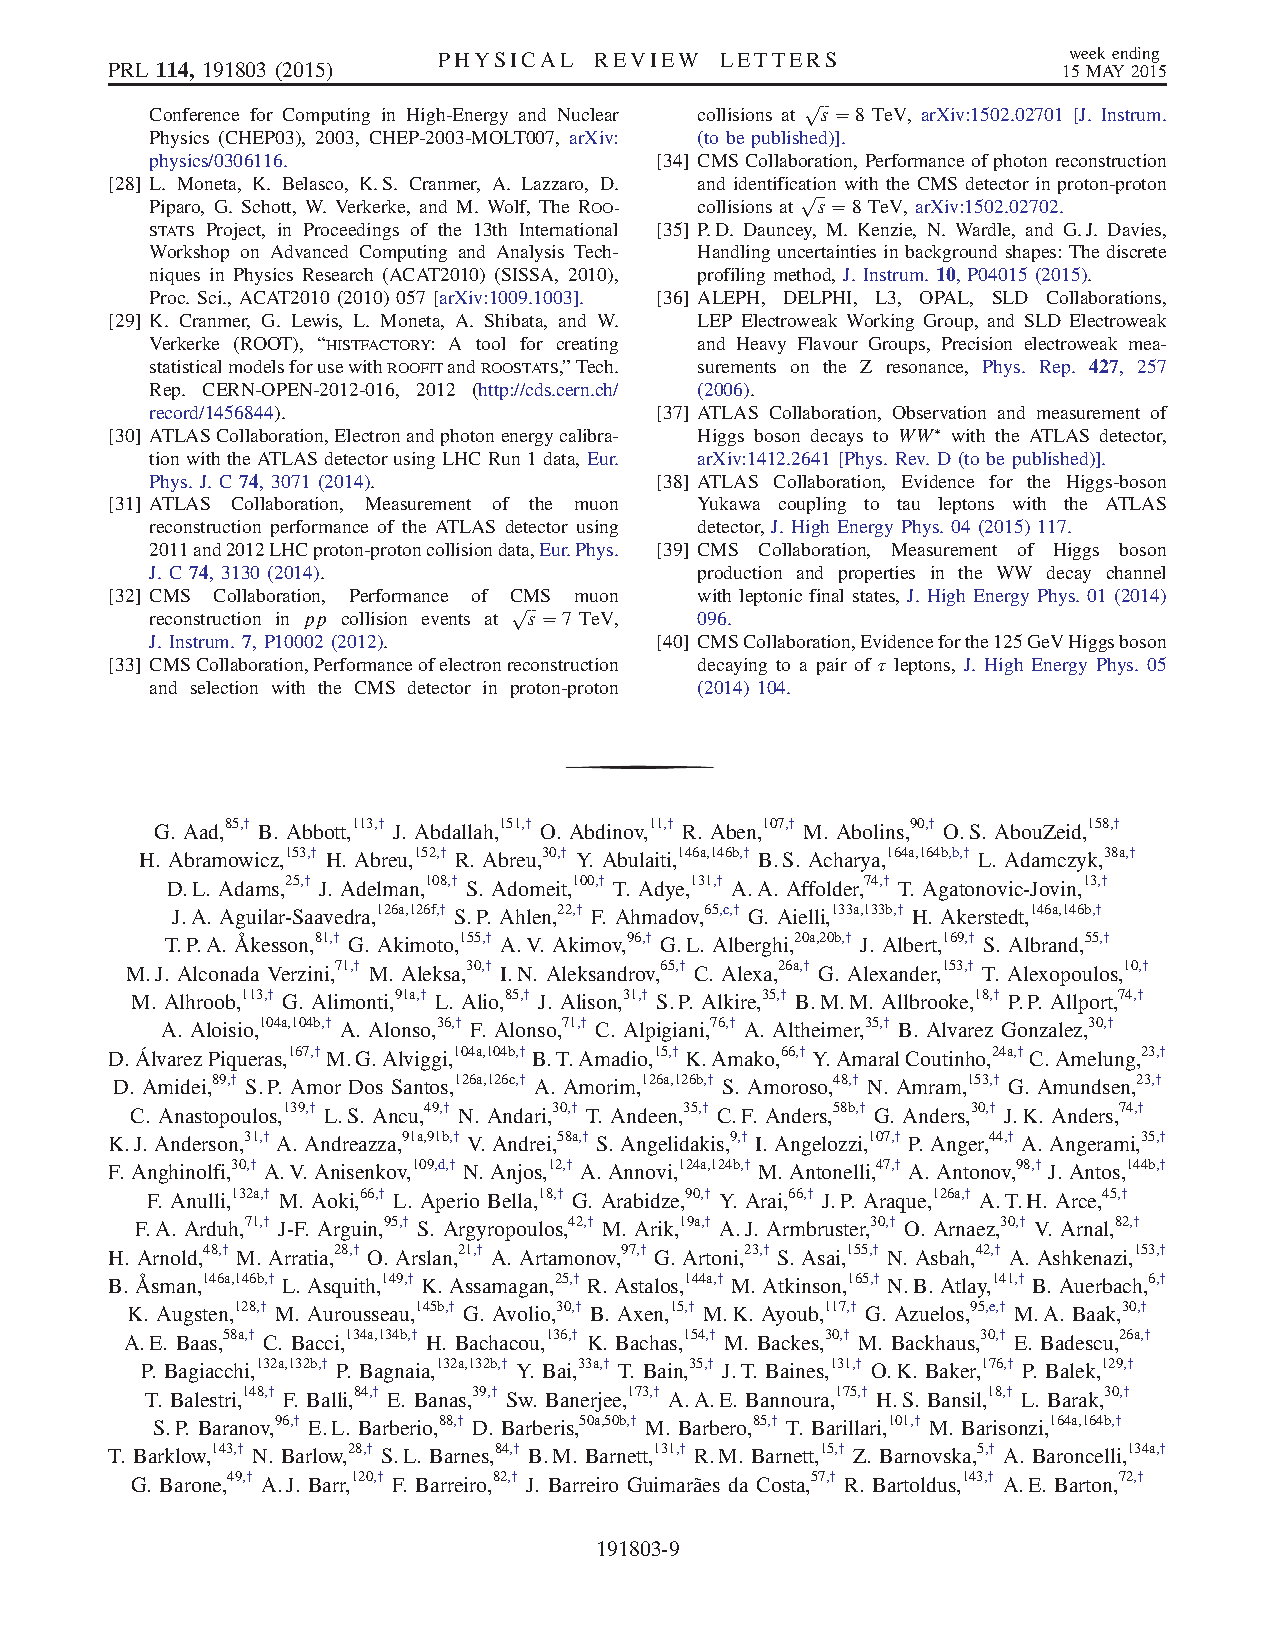
\includegraphics[height=\textheight]{figures/aad_combined_2015_authors_01}}%
\only<2>{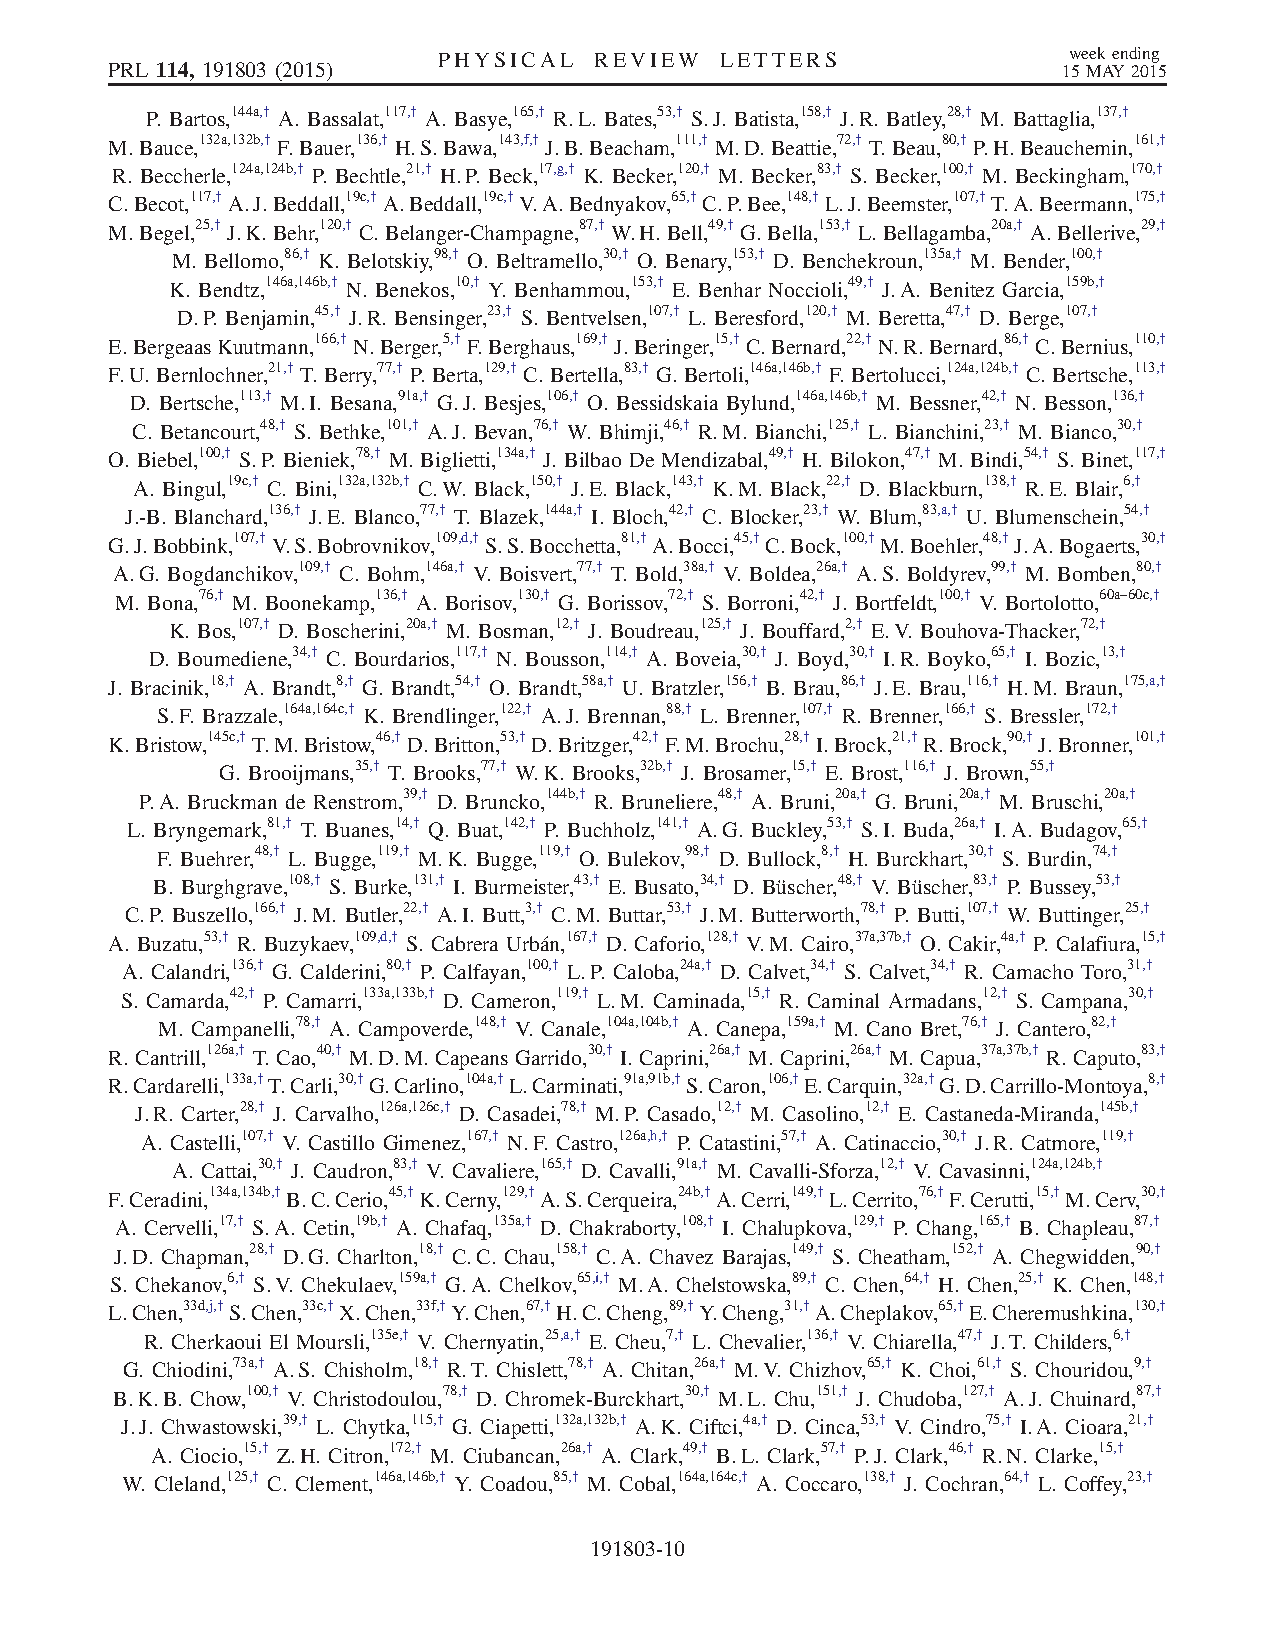
\includegraphics[height=\textheight]{figures/aad_combined_2015_authors_02}}%
\only<3>{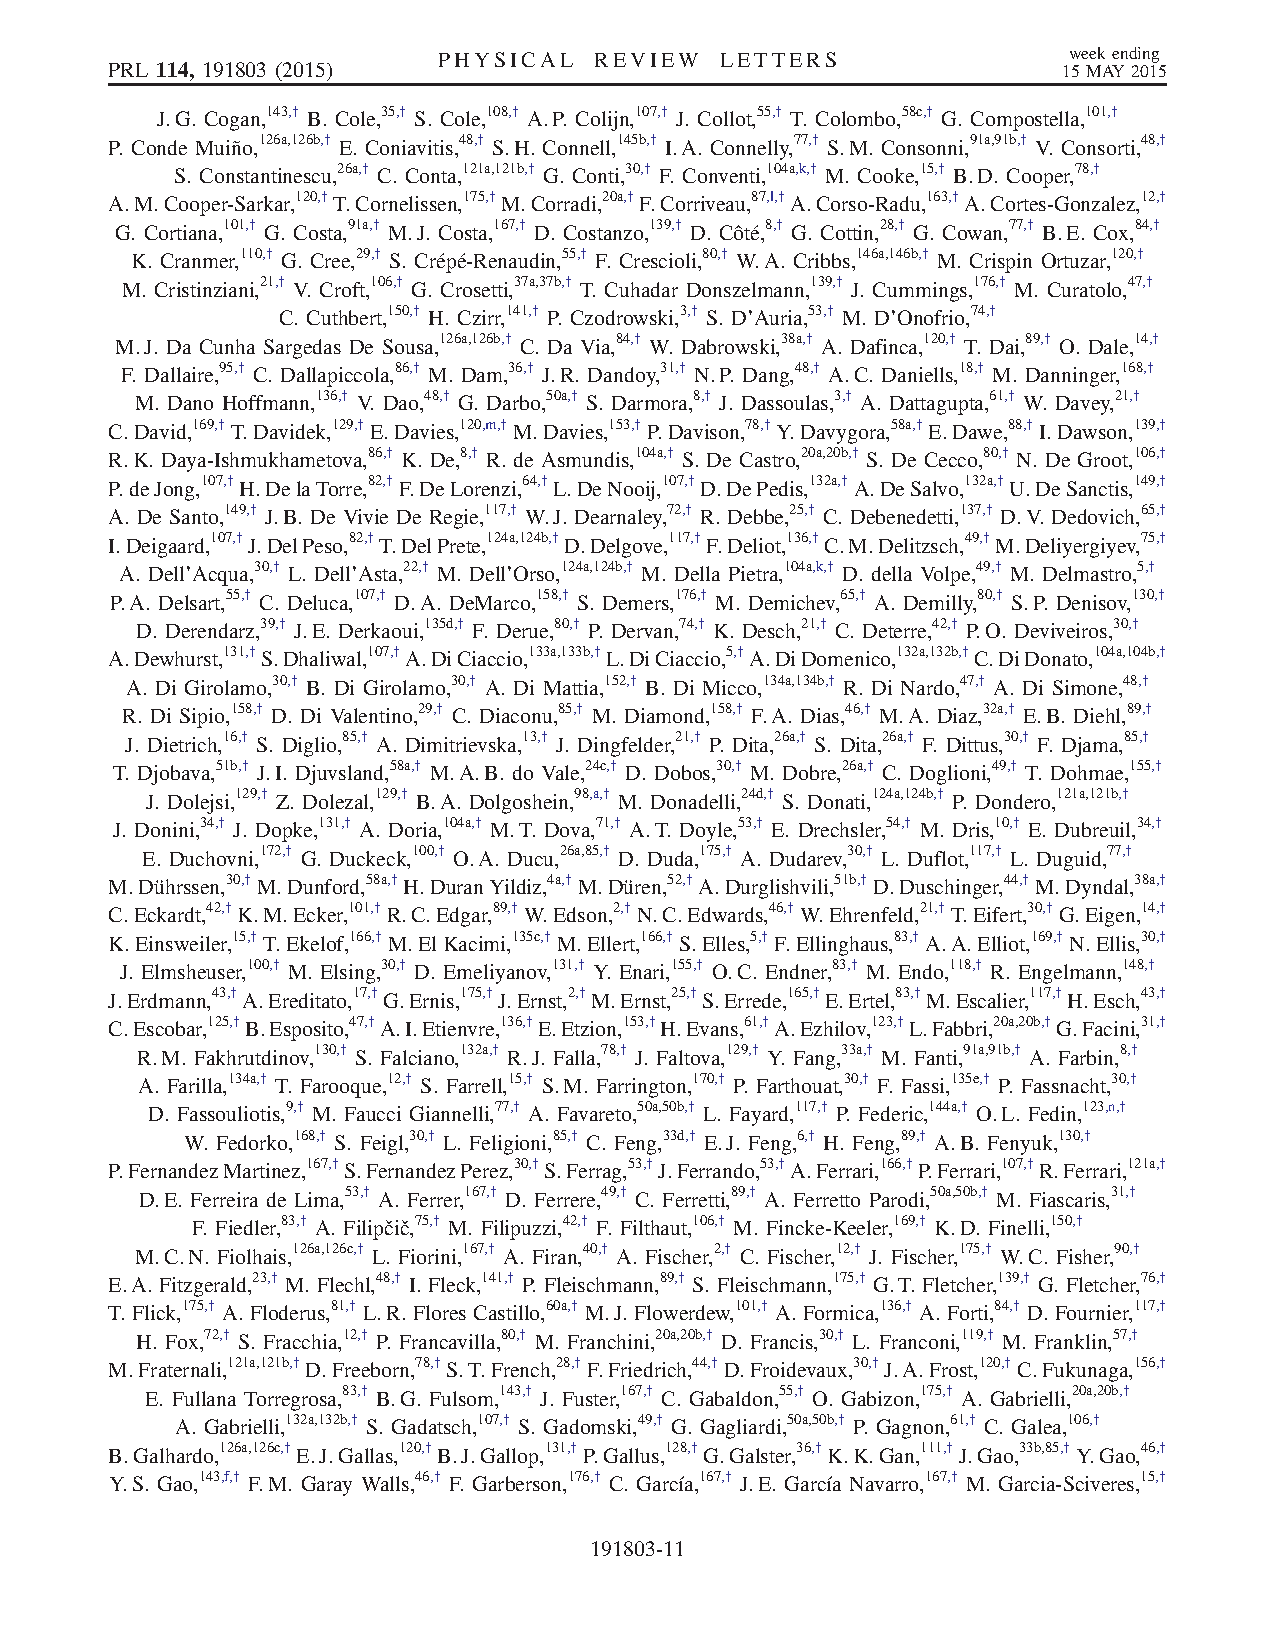
\includegraphics[height=\textheight]{figures/aad_combined_2015_authors_03}}%
\only<4>{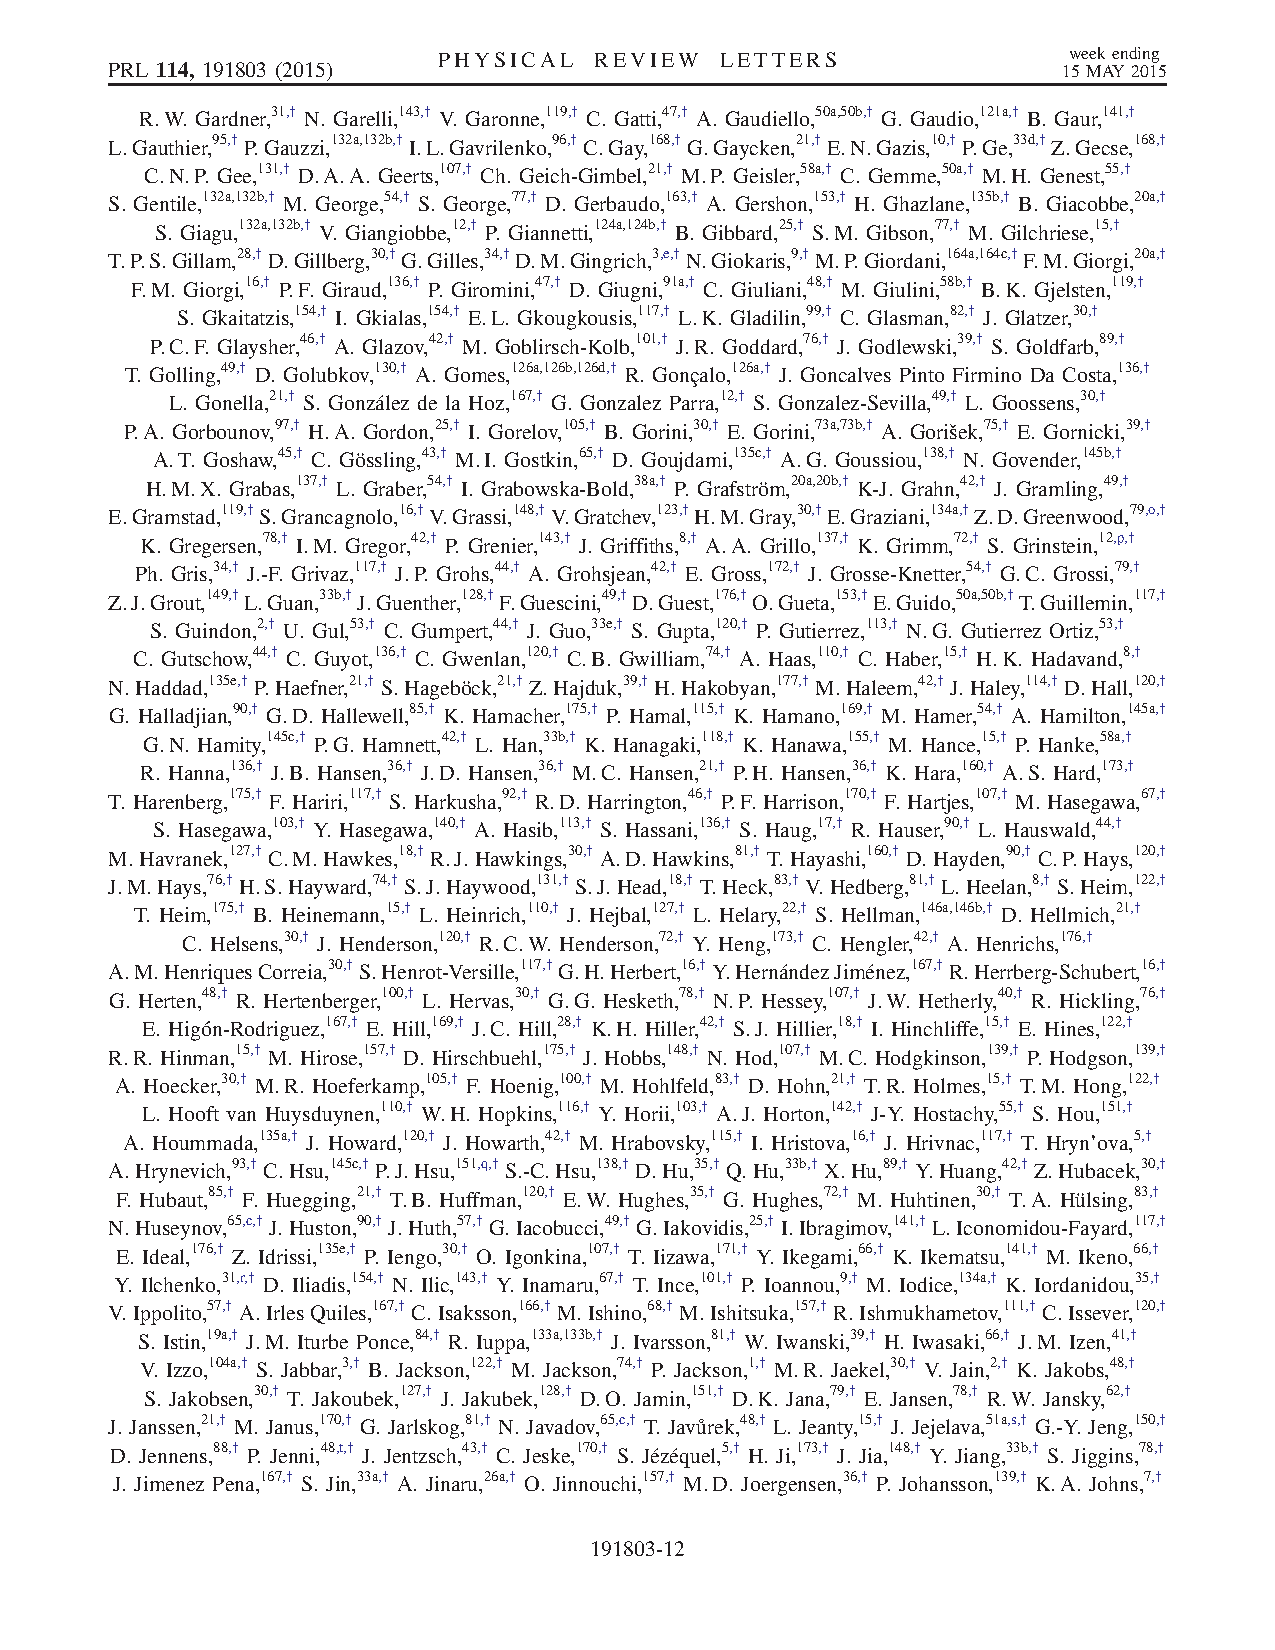
\includegraphics[height=\textheight]{figures/aad_combined_2015_authors_04}}%
\only<5>{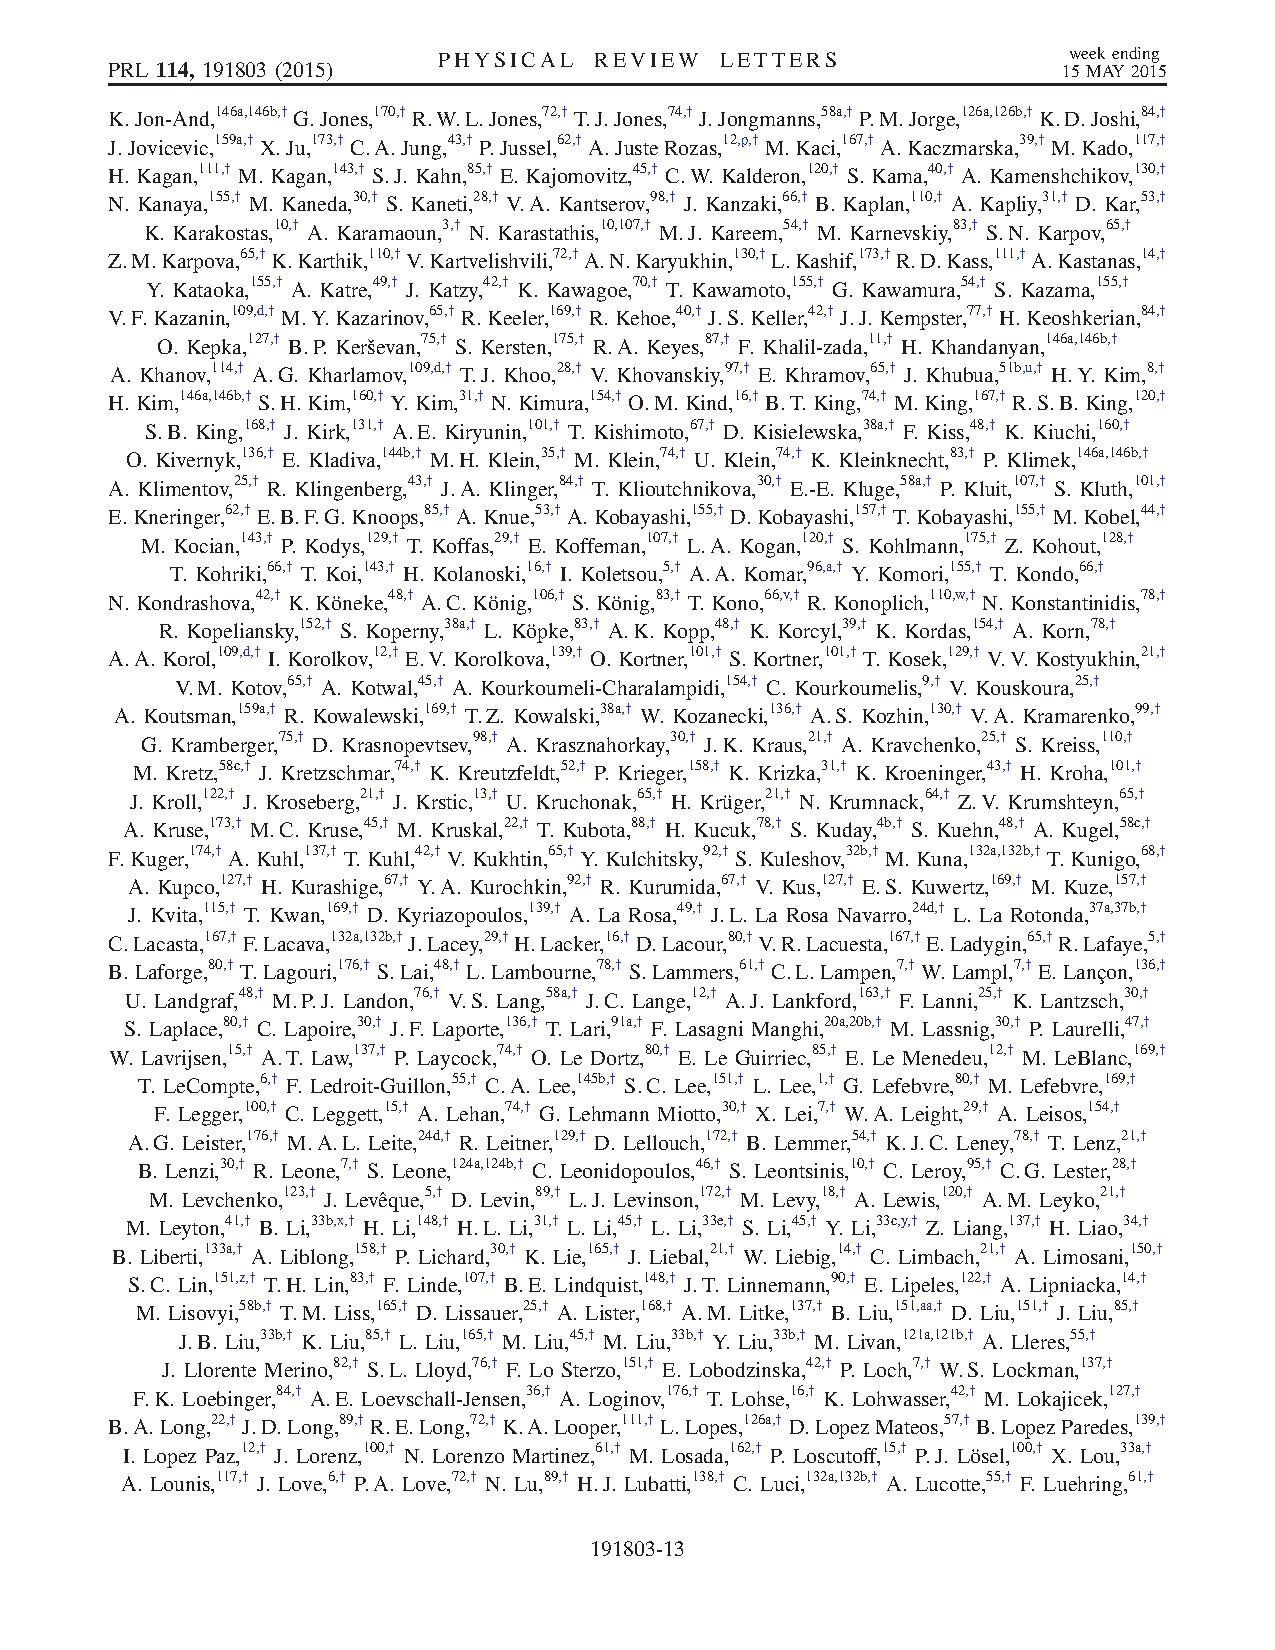
\includegraphics[height=\textheight]{figures/aad_combined_2015_authors_05}}%
\only<6>{
\includegraphics[height=\textheight]{figures/aad_combined_2015_authors_06}}%
\only<7>{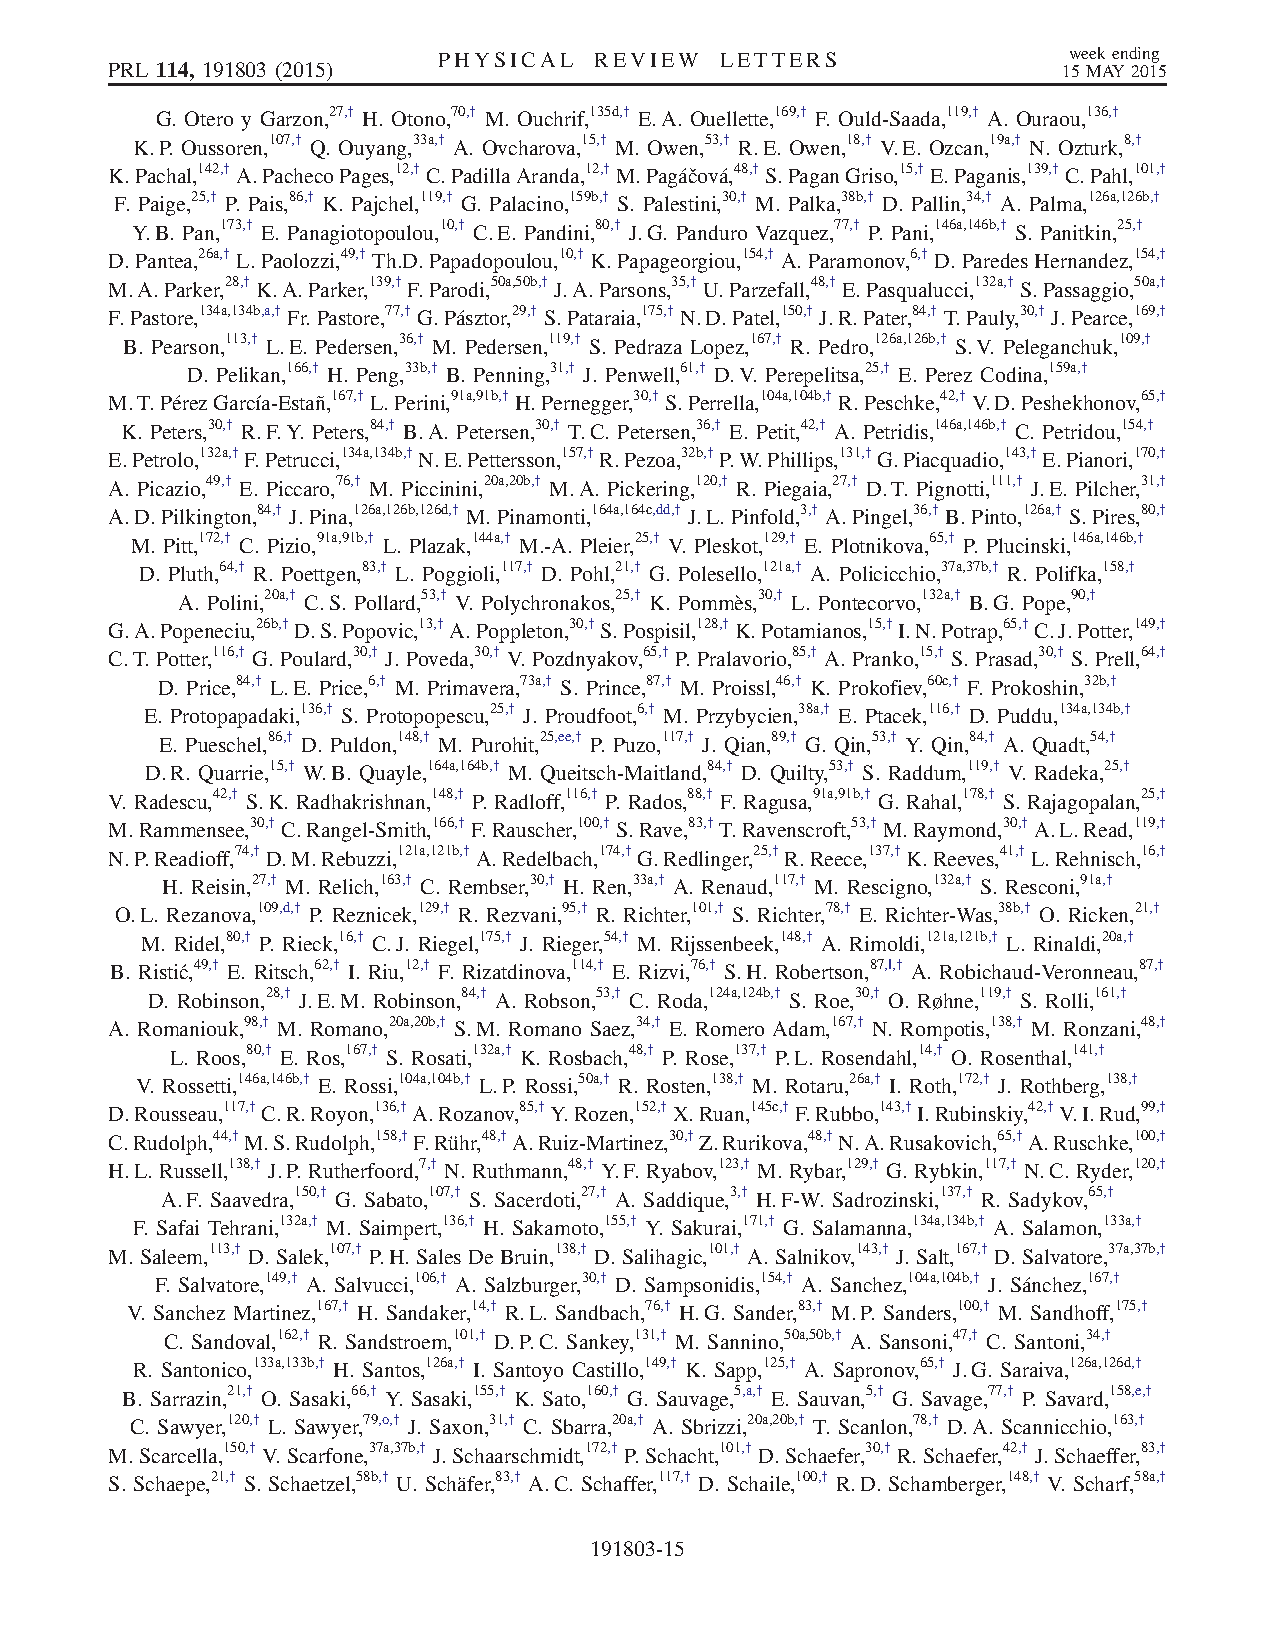
\includegraphics[height=\textheight]{figures/aad_combined_2015_authors_07}}%
\only<8>{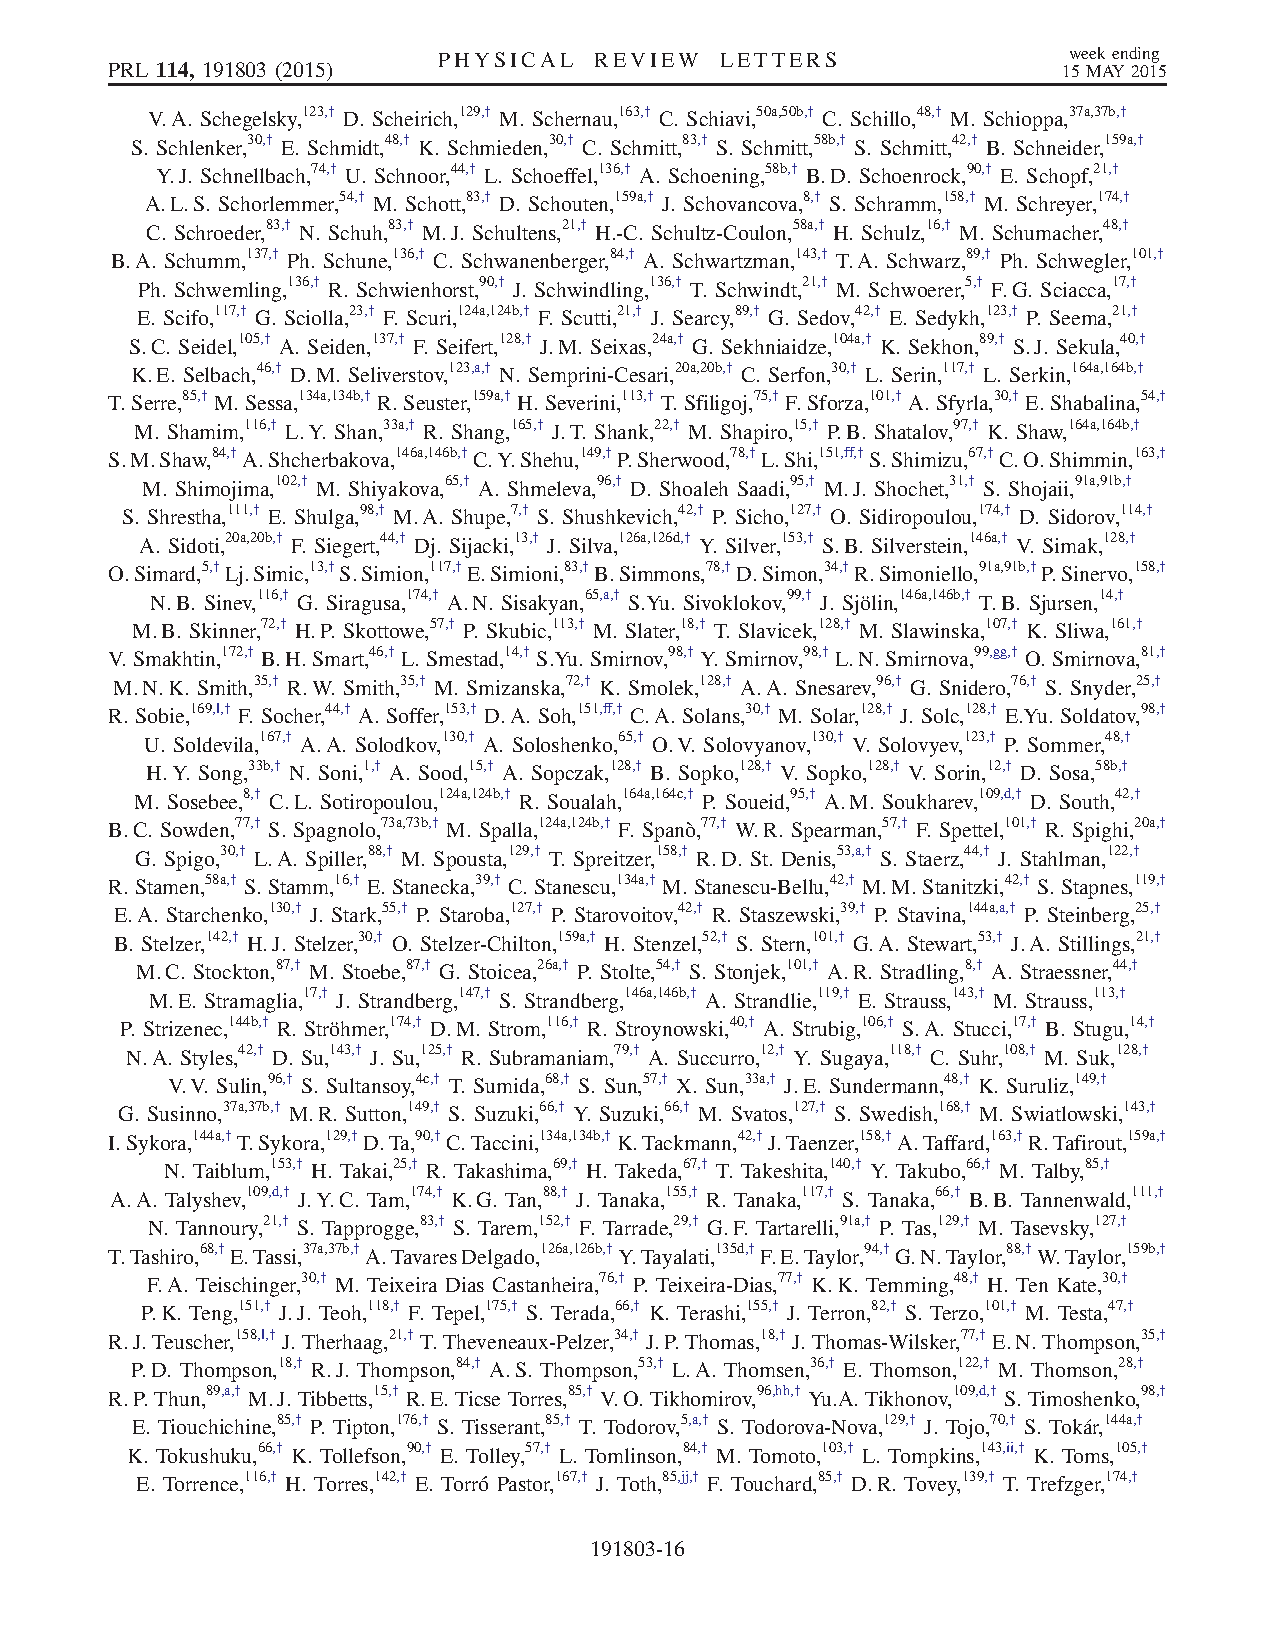
\includegraphics[height=\textheight]{figures/aad_combined_2015_authors_08}}%
\only<9>{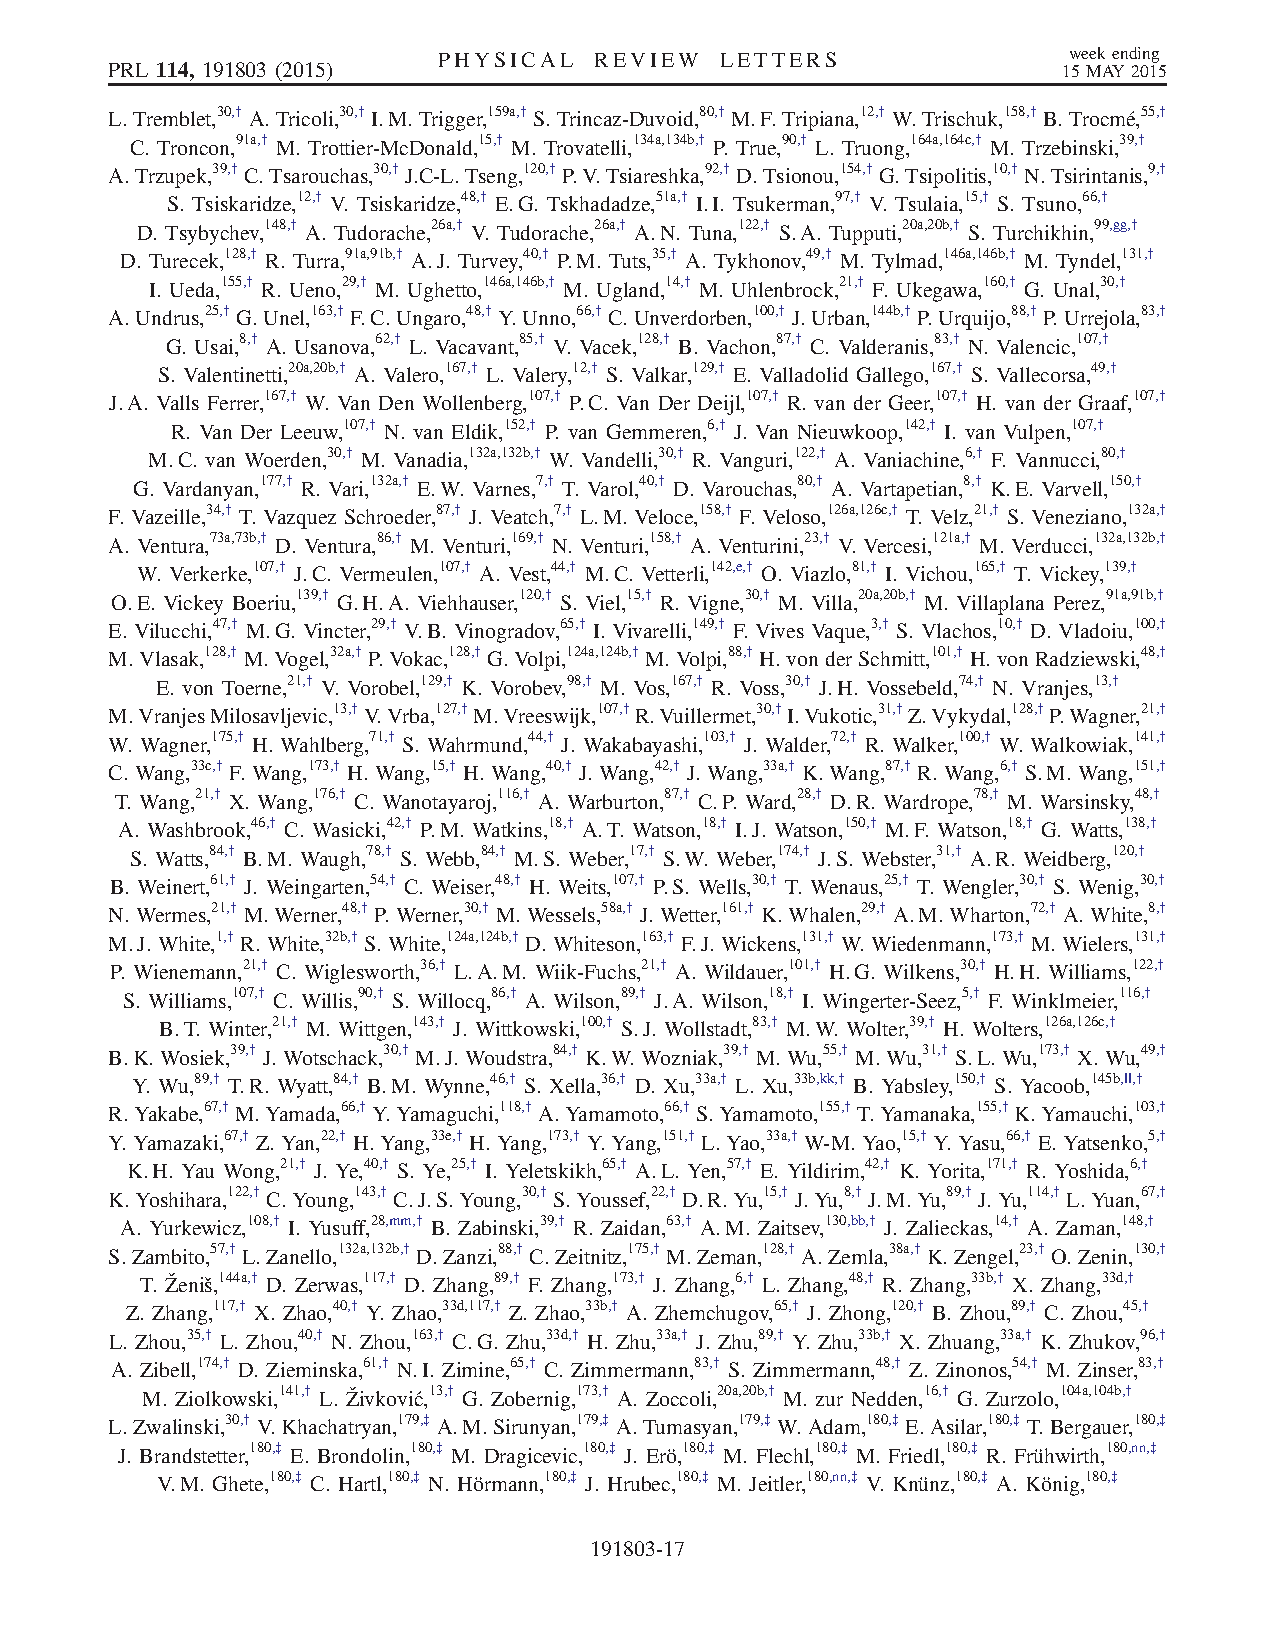
\includegraphics[height=\textheight]{figures/aad_combined_2015_authors_09}}%
\only<10>{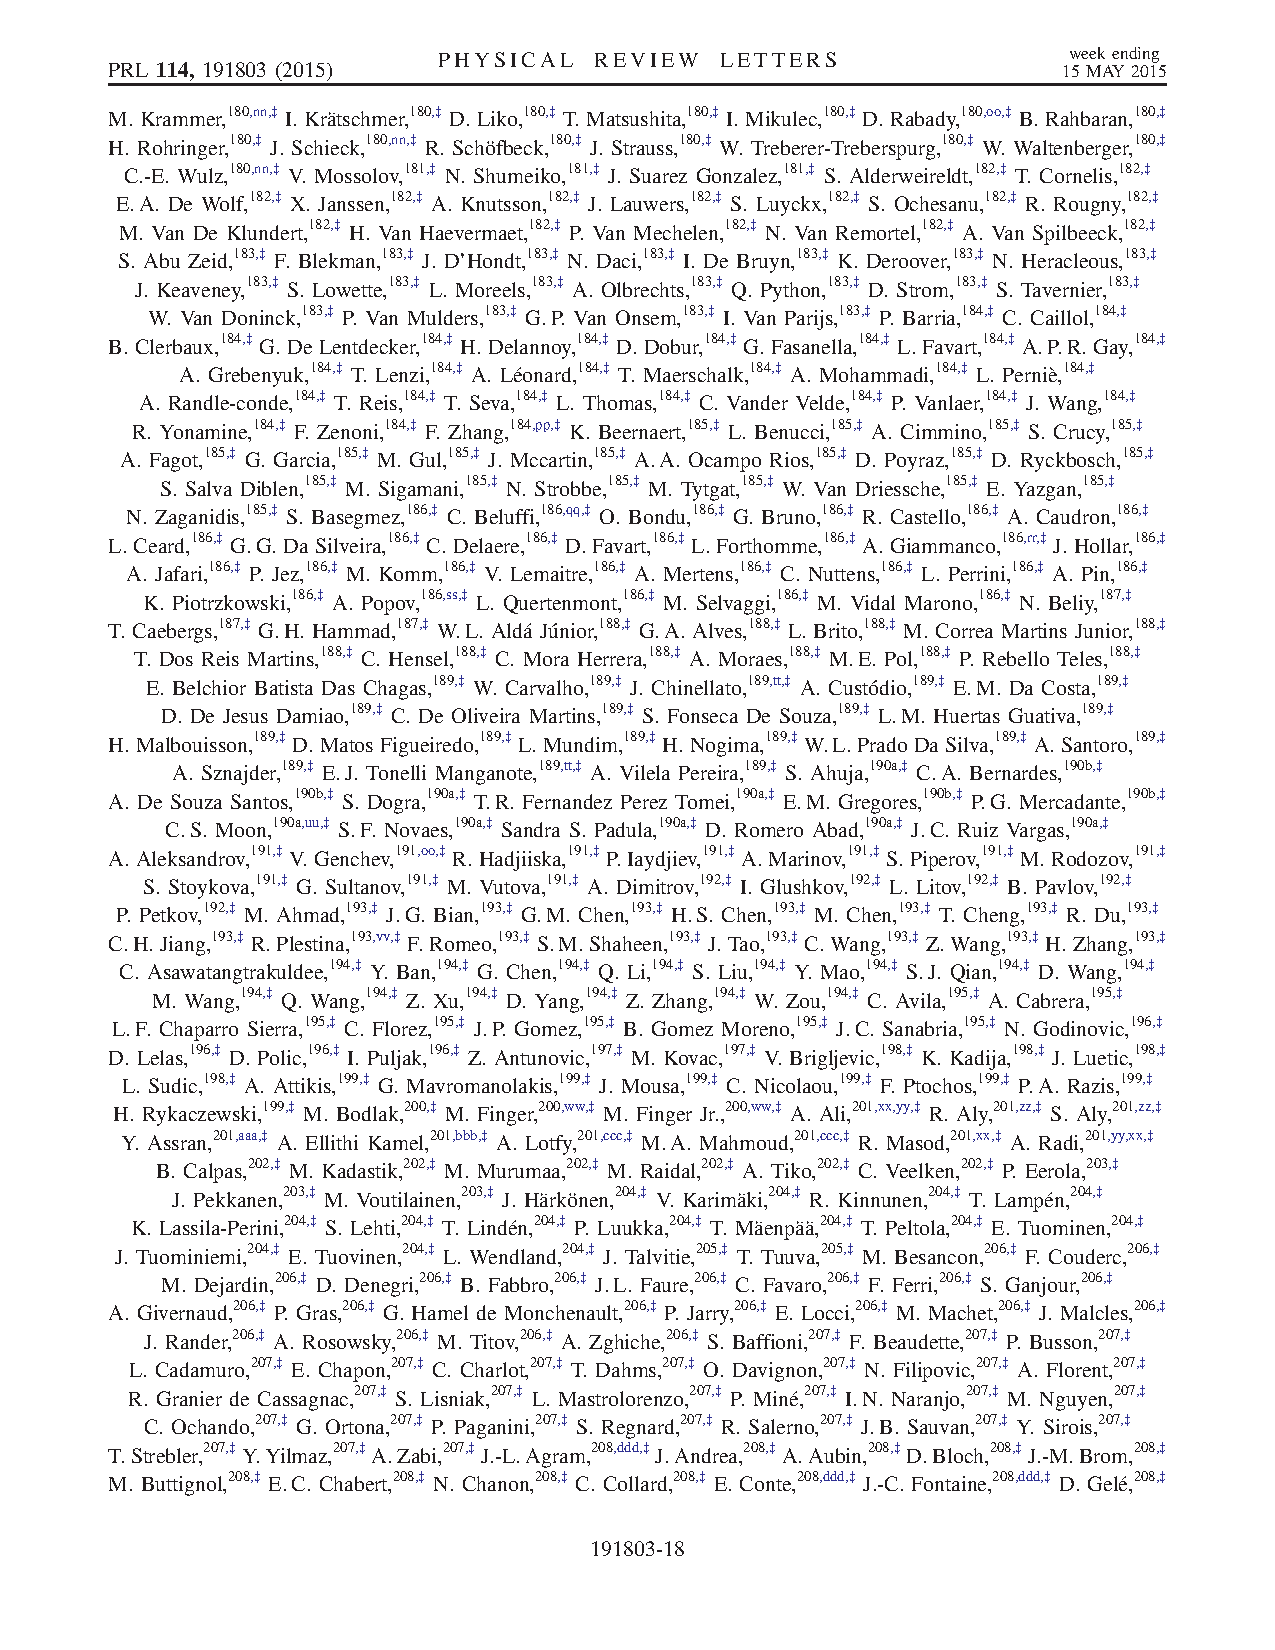
\includegraphics[height=\textheight]{figures/aad_combined_2015_authors_10}}%
\only<11>{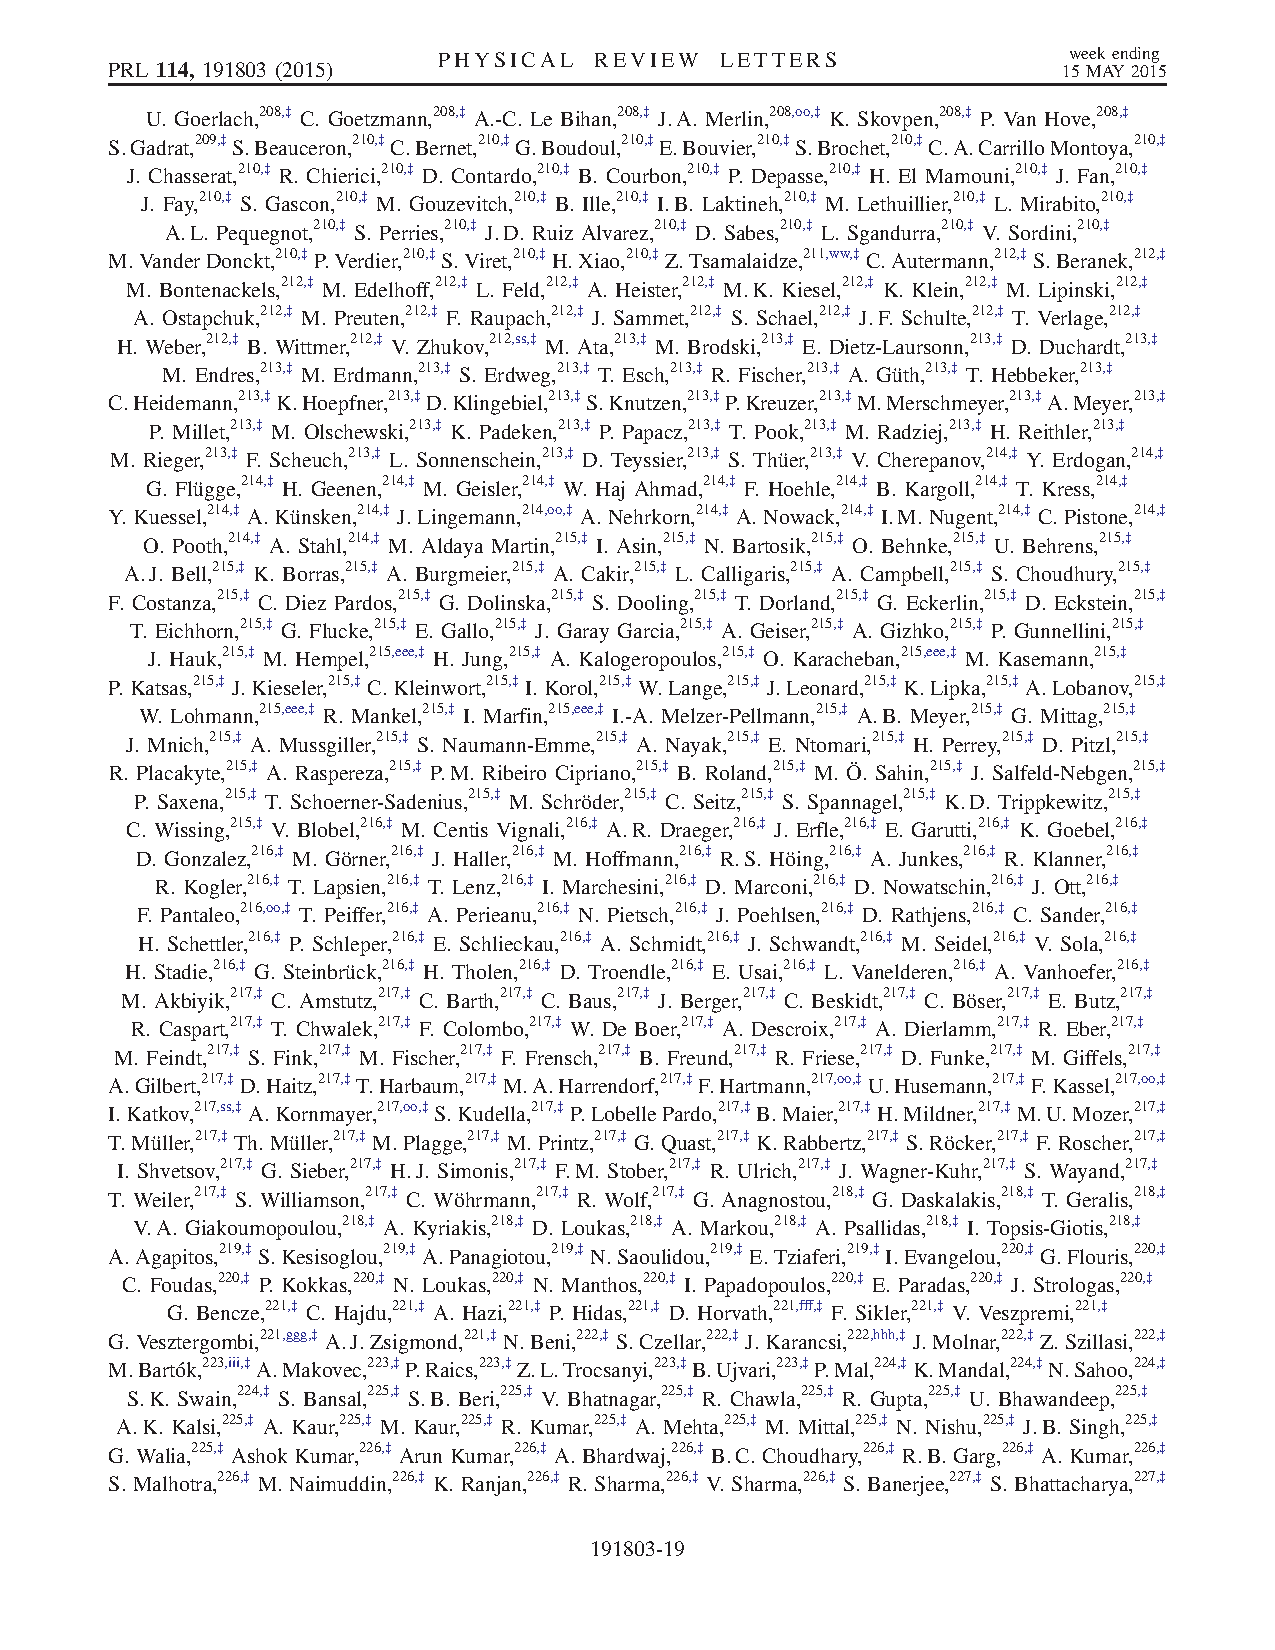
\includegraphics[height=\textheight]{figures/aad_combined_2015_authors_11}}%
\only<12>{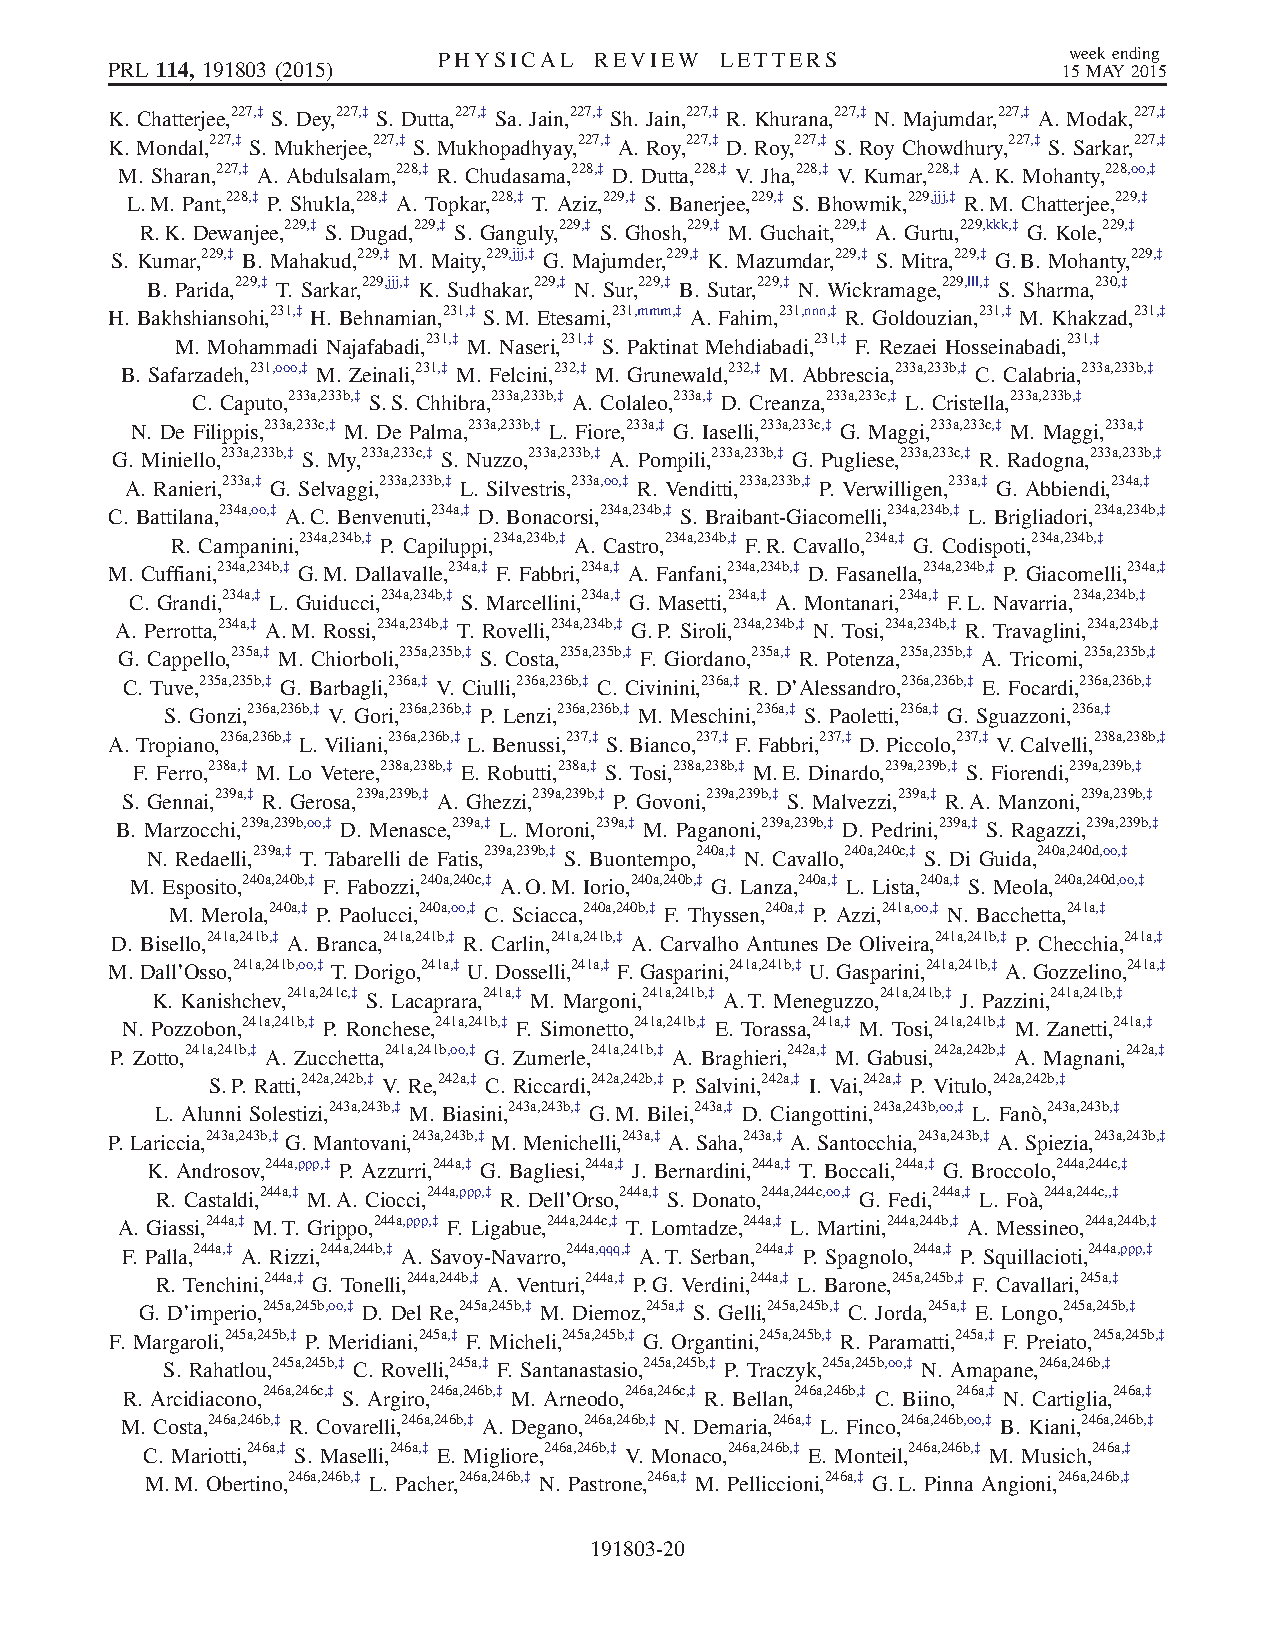
\includegraphics[height=\textheight]{figures/aad_combined_2015_authors_12}}%
\only<13>{\includegraphics<13>[height=\textheight]{figures/aad_combined_2015_authors_13}}%
\only<14>{\includegraphics<14>[height=\textheight]{figures/aad_combined_2015_authors_14}}%
\only<15>{\includegraphics<15>[height=\textheight]{figures/aad_combined_2015_authors_15}}%
\only<16>{\includegraphics<16>[height=\textheight]{figures/aad_combined_2015_authors_16}}%
\only<17>{\includegraphics<17>[height=\textheight]{figures/aad_combined_2015_authors_17}}%
\only<18>{\includegraphics<18>[height=\textheight]{figures/aad_combined_2015_authors_18}}%
\only<19>{\includegraphics<19>[height=\textheight]{figures/aad_combined_2015_authors_19}}%
\only<20>{\includegraphics<20>[height=\textheight]{figures/aad_combined_2015_authors_20}}%
\only<21>{\includegraphics<21>[height=\textheight]{figures/aad_combined_2015_authors_21}}%
\only<22>{\includegraphics<22>[height=\textheight]{figures/aad_combined_2015_authors_22}}%
\only<23>{\includegraphics<23>[height=\textheight]{figures/aad_combined_2015_authors_23}}%
\only<24>{\includegraphics<24>[height=\textheight]{figures/aad_combined_2015_authors_24}}%
\only<25>{\includegraphics<25>[height=\textheight]{figures/aad_combined_2015_authors_25}}
\end{center}

\end{frame}
%%%%%%%%%%%%%%%%%%%%%%%%%
\begin{frame}

\begin{center}
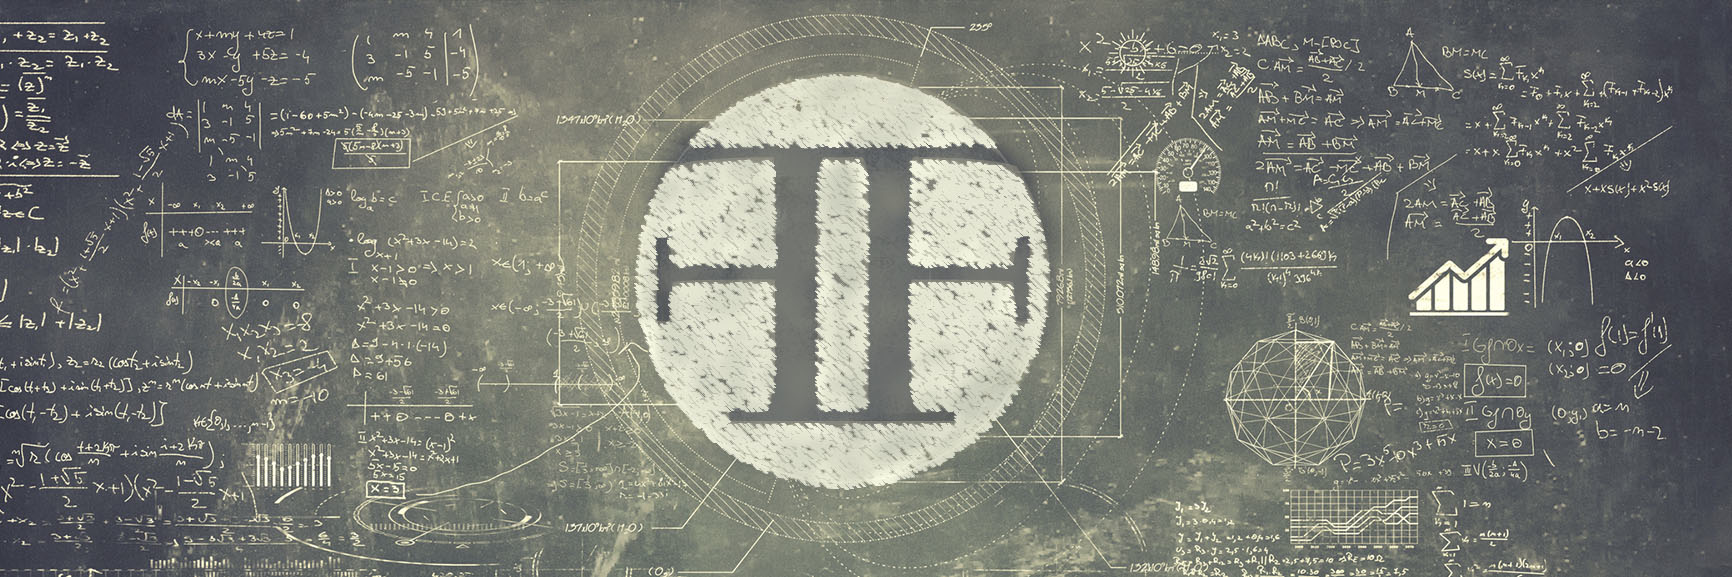
\includegraphics[width=\textwidth]{figures/ffc_masthead}
\Large{Fragile Families Challenge}
\end{center}

\end{frame}
%%%%%%%%%%%%%%%%%%%%%%%%%%%
\begin{frame}
\centering
\begin{tikzpicture}[x = .5\textwidth, y = .5\textheight]
\node at (-1,-1) {};
\node at (1,1) {};
\node[font = \Large] at (0,.8) {An overly simple view of stratification research.};
\onslide<1-1>{
	\node[font = \Huge] at (0,.5) {$Y = \white{\underbrace{\black{\E\left(Y\mid \vec{X}\right)}}} + \epsilon$};
}
\onslide<8->{
	\node[font = \Huge] at (0,.5) {$Y = \underbrace{\E\left(Y\mid \vec{X}\right)} + \hspace{5pt}\epsilon$};
}
\onslide<2-3>{
	\node[font = \Huge] at (0,.5) {$\blue{Y} = \white{\underbrace{\black{\E\left(Y\mid \vec{X}\right)}}} + \epsilon$};
}
\onslide<4-5,7>{
	\node[font = \Huge] at (0,.5) {$Y = \blue{\underbrace{\E\left(Y\mid \vec{X}\right)}} + \epsilon$};
}
\onslide<6>{
	\node[font = \Huge] at (0,.5) {$Y = \blue{\underbrace{\beta_1X_1 + \beta_2X_2}} + \epsilon$};
}
\onslide<8-9>{
	\node[font = \Huge] at (0,.5) {$Y = \underbrace{\E\left(Y\mid \vec{X}\right)} +\blue{\hspace{5pt}\epsilon}$};
}
\onslide<2-3>{
	\node[font = \Large,blue,anchor=west] (attainment) at (-1,.2) {\bblue{Attainment}};
	\draw[->, line width = 1.5pt, blue] (-.6,0.4) -- (attainment);
}
\onslide<3-3>{
	\node[font = \Large,blue,anchor = west,align=left] (achievement) at (-1,0) {-- Academic\\\hspace{13pt}achievement};
	\node[font = \Large,blue,anchor = west] (occupation) at (-1,-.22) {-- Occupation};
	\node[font = \Large,blue,anchor = west] (income) at (-1,-.37) {-- Income};
}
\onslide<4-9>{
	\node[font = \Large,black,anchor = west,align=left] (achievement) at (-1,0) {-- Academic\\\hspace{13pt}achievement};
	\node[font = \Large,black,anchor = west] (occupation) at (-1,-.22) {-- Occupation};
	\node[font = \Large,black,anchor = west] (income) at (-1,-.37) {-- Income};
}
\onslide<4->{
	\node[font = \Large,anchor=west] (attainment) at (-1,.2) {\textbf{Attainment}};
	\draw[->, line width = 1.5pt] (-.6,0.4) -- (attainment);
}
\onslide<4-7>{
	\node[font = \Large,blue,anchor=north,align=center] (predictable) at (0.04,.15) {\bblue{Predictable}\\\bblue{component}};
	\draw[->, line width = 1.5pt, blue] (0.04, 0.25) -- (predictable);
}
\onslide<8->{
	\node[font = \Large,anchor=north,align=center] (predictable) at (0.04,.15) {\textbf{Predictable}\\\textbf{component}};
	\draw[->, line width = 1.5pt] (0.04, 0.25) -- (predictable);
}
\onslide<8-9>{
	\node[font = \Large,align=center,blue] (unpredictable) at (.7,.1) {\bblue{Unpredictable}\\\bblue{component}};
	\draw[->, line width = 1.5pt, blue] (.63,0.4) -- (unpredictable);
}
\onslide<10->{
	\node[font = \Large,align=center] (unpredictable) at (.7,.1) {\textbf{Unpredictable}\\\textbf{component}};
	\draw[->, line width = 1.5pt] (0.63,0.4) -- (unpredictable);
}
\onslide<10->{
	\node[font = \Large,anchor = west] at (-1.05,-.25) {Theories focus on the predictable component, but};
}
\onslide<10->{
	\node[font = \Large,anchor = west] at (-1.05,-.4) {empirically the unpredictable component dominates};
}
\end{tikzpicture}
\end{frame}
%%%%%%%%%%%%%%%%%%%%%%%%%%%%%%%
\begin{frame}

\begin{center}
\Huge{
$ \hat{y} \quad \& \quad \hat{\beta}$
}
\end{center}

\vfill
\tiny{Mullainathan and Spiess (2017)}
\end{frame}
%%%%%%%%%%%%%%%%%%%%%%%%%%
\begin{frame}

Why should we care about the predictability of social outcomes?\pause
\begin{itemize}
\item Scientific reasons \pause
\begin{itemize}
\item Basic social fact \pause
\item Discovery \pause
\end{itemize}
\item Policy reasons
\begin{center}
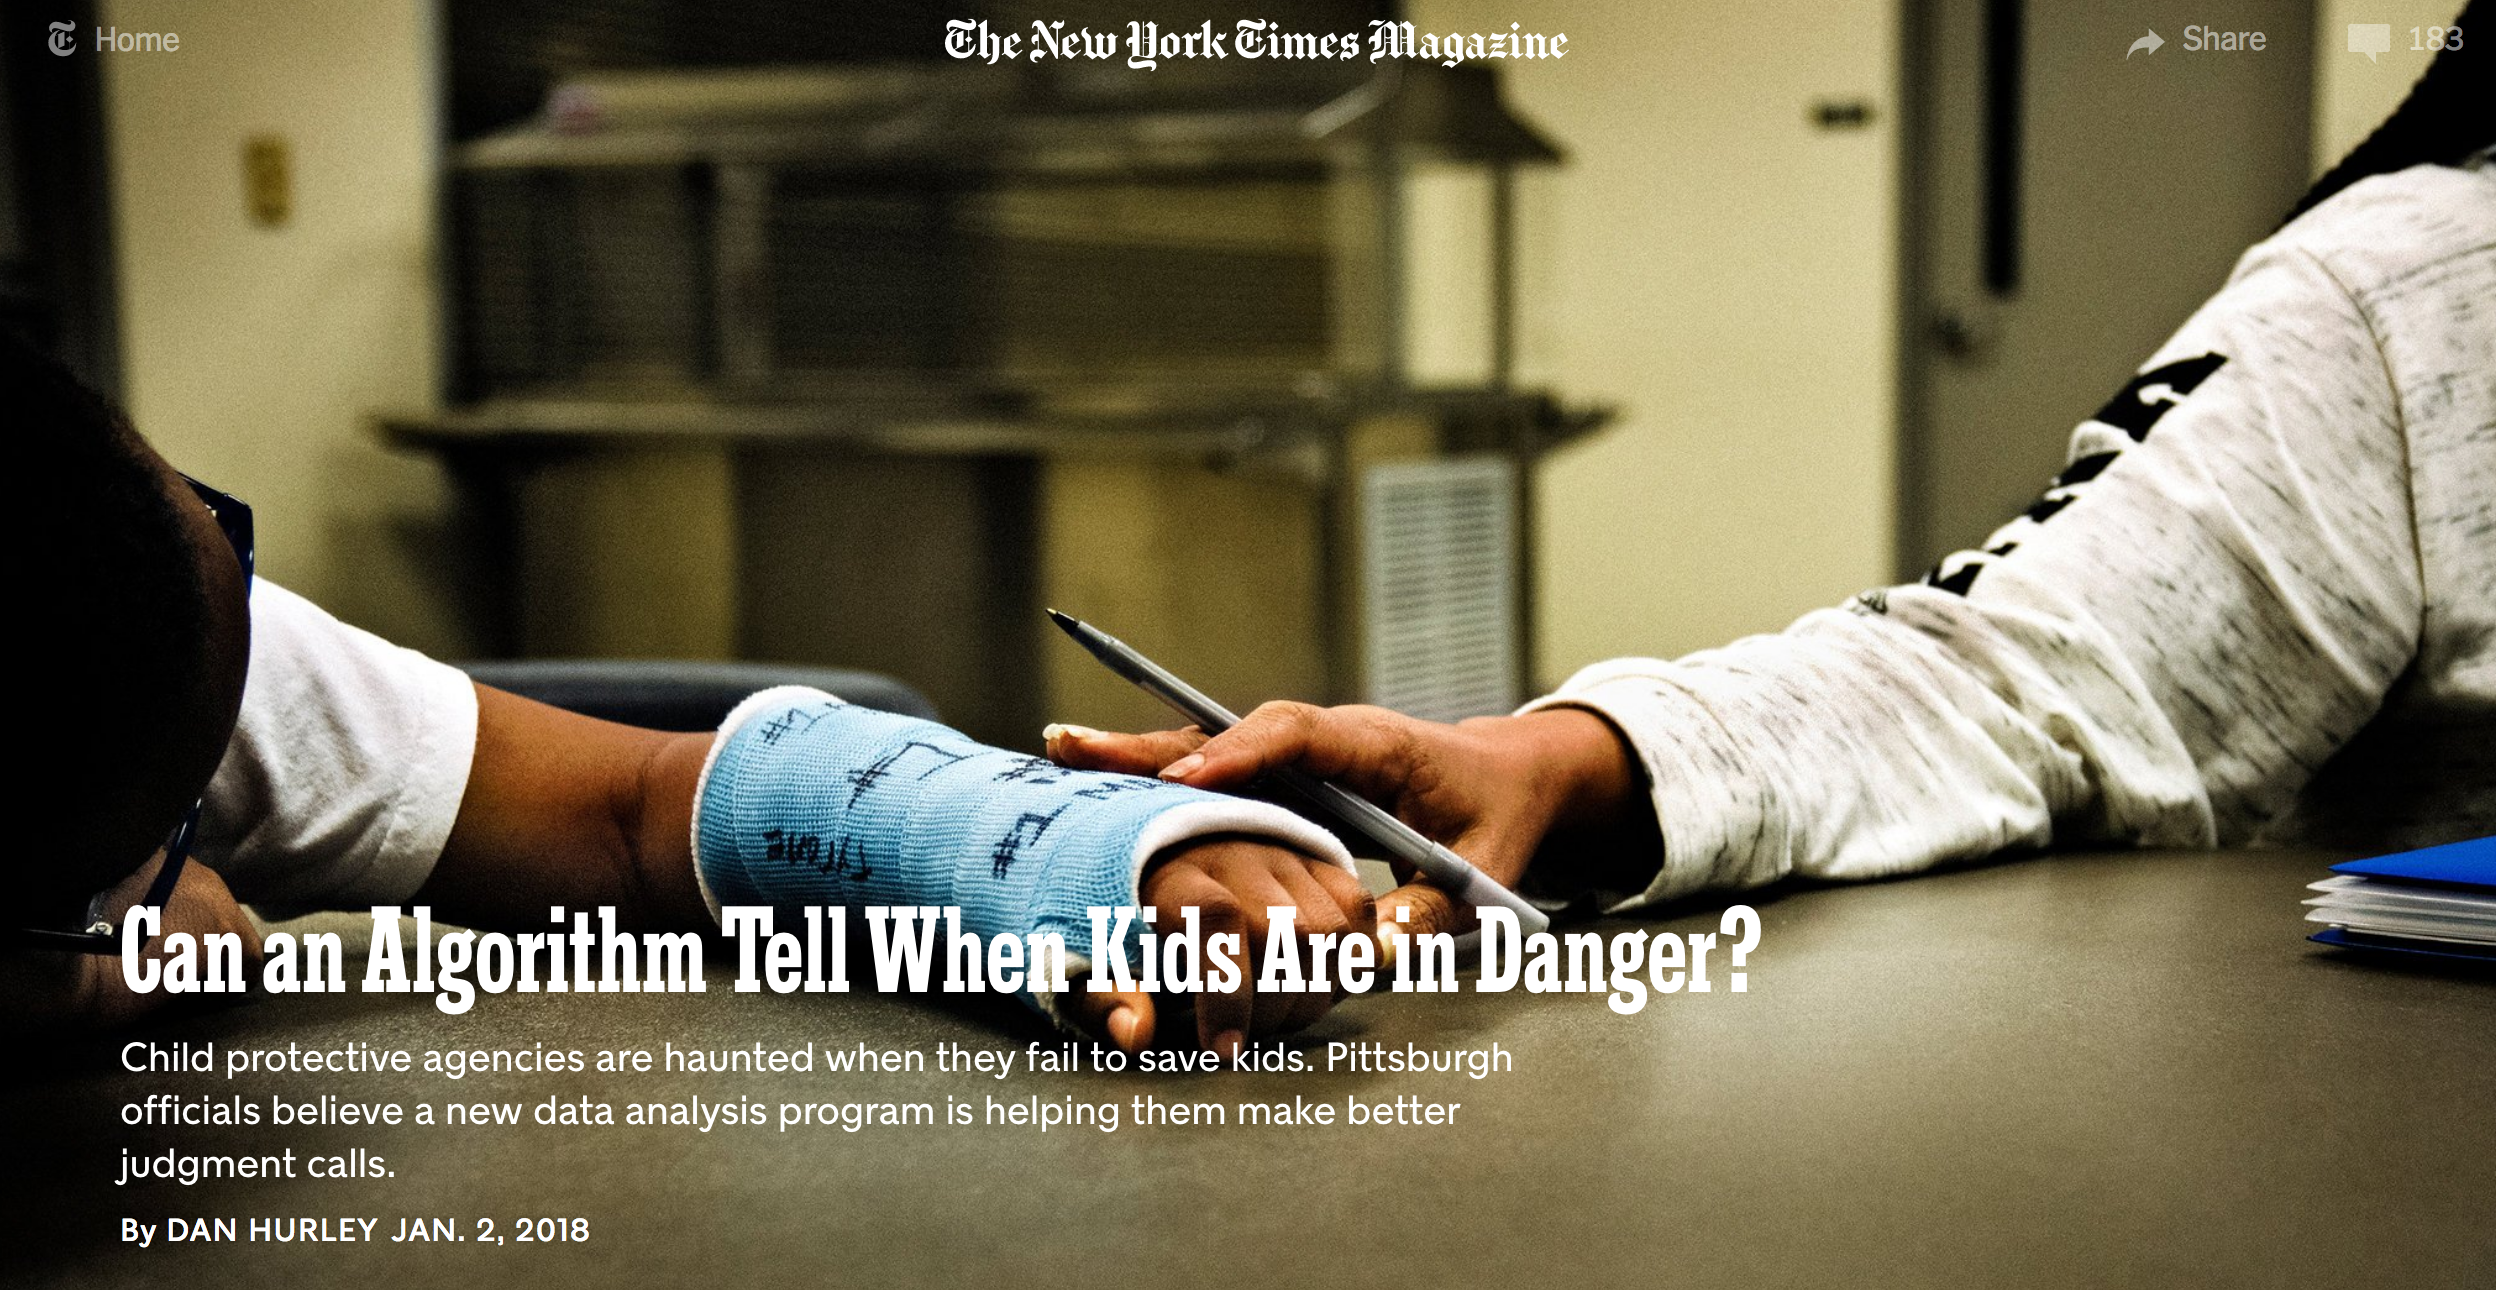
\includegraphics[width=0.8\textwidth]{figures/hurley_can_2018_title} 
\end{center}
\end{itemize}

\end{frame}
%%%%%%%%%%%%%%%%%%%%%%%%%
\begin{frame}

\begin{center}

\includegraphics[width=\textwidth]{figures/ff_logo}
\end{center}

\begin{itemize}
\item Birth cohort panel study
\item $\approx$ 5,000 children born in 20 U.S. cities with an over-sample of non-marital births
\item Followed from birth through age 15
\item Already used in hundreds of papers and dozens of dissertations
\end{itemize}

\end{frame}
%%%%%%%%%%%%%%%%%%%%%%%%%%%
\begin{frame}

\begin{center}
\only<1>{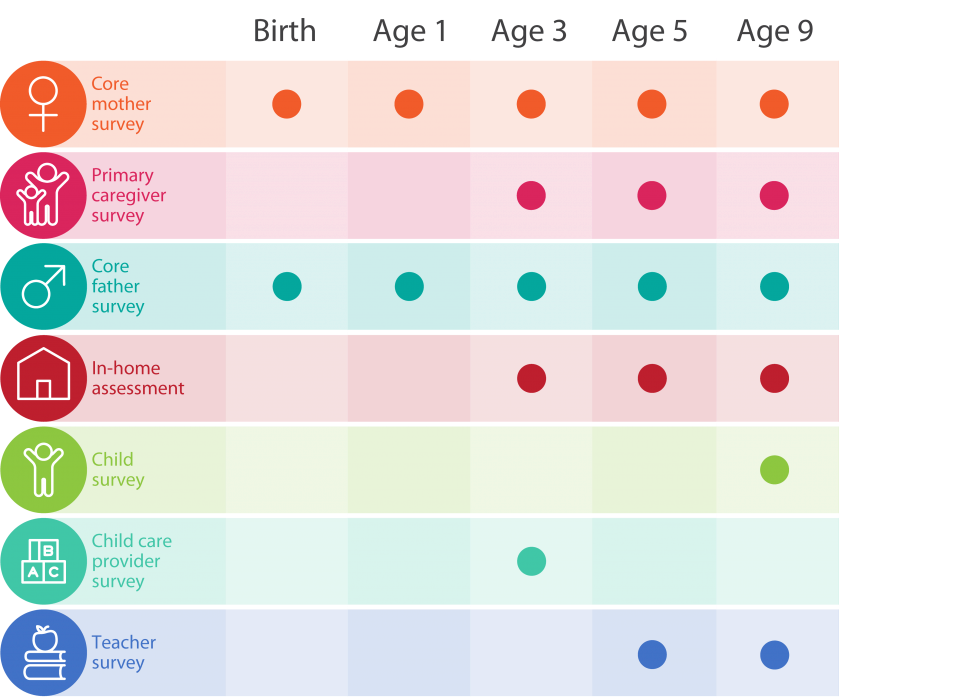
\includegraphics[width=0.8\textwidth]{figures/ff_design_public_b9}}
\only<2>{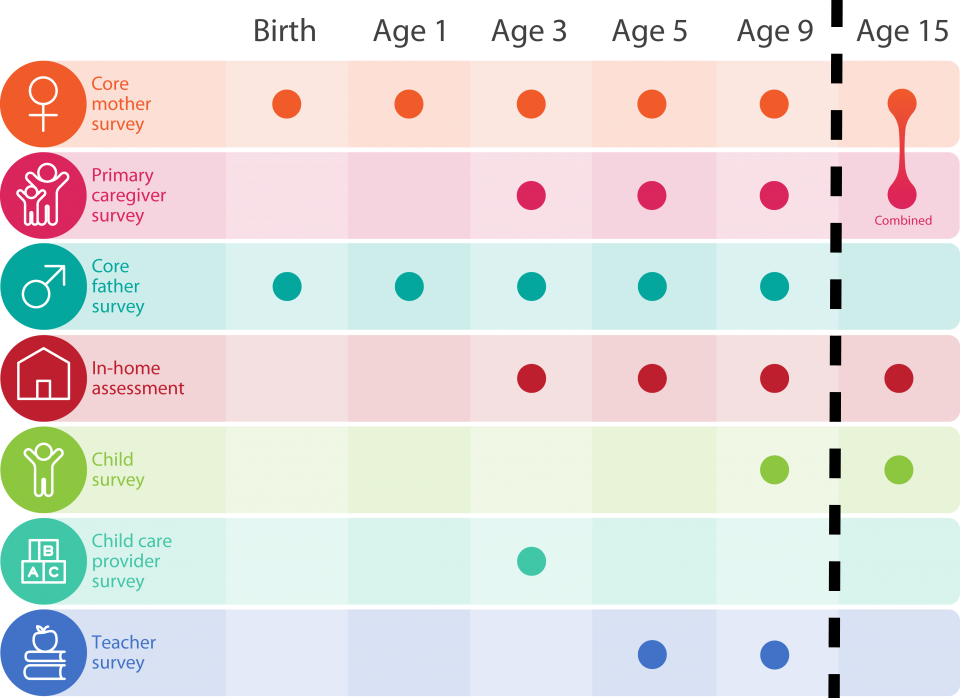
\includegraphics[width=0.8\textwidth]{figures/ff_design_public2}}
\end{center}

\end{frame}
%%%%%%%%%%%%%%%%%%%%%%%%%
\begin{frame}

\begin{center}
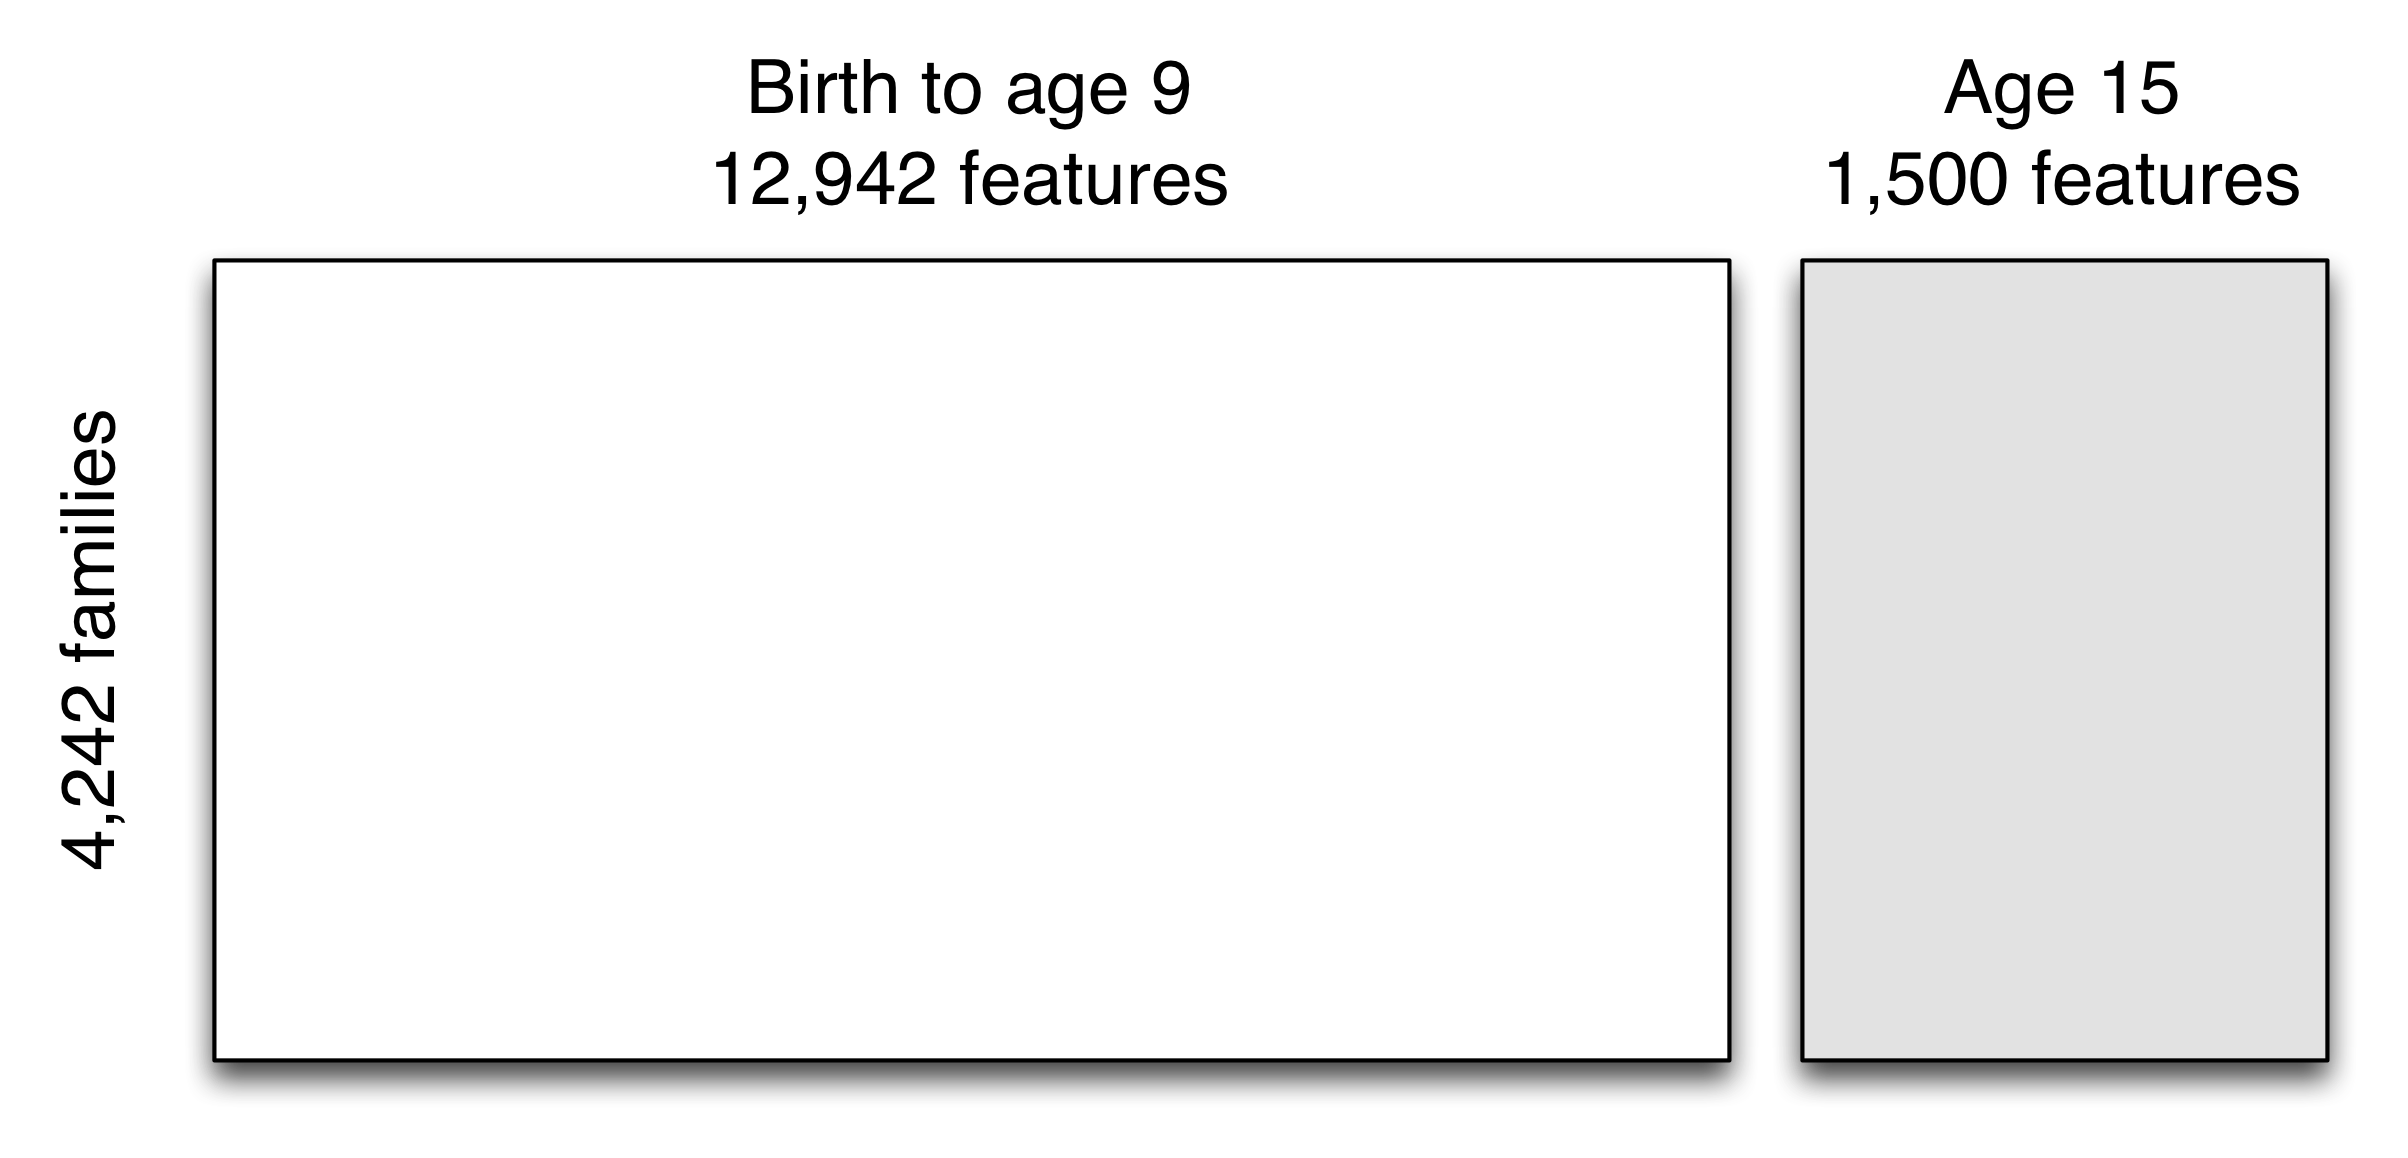
\includegraphics[width=\textwidth]{figures/ff_design_matrix_ml}
\end{center}

\end{frame}
%%%%%%%%%%%%%%%%%%%%%%%%%
\begin{frame}

\begin{center}
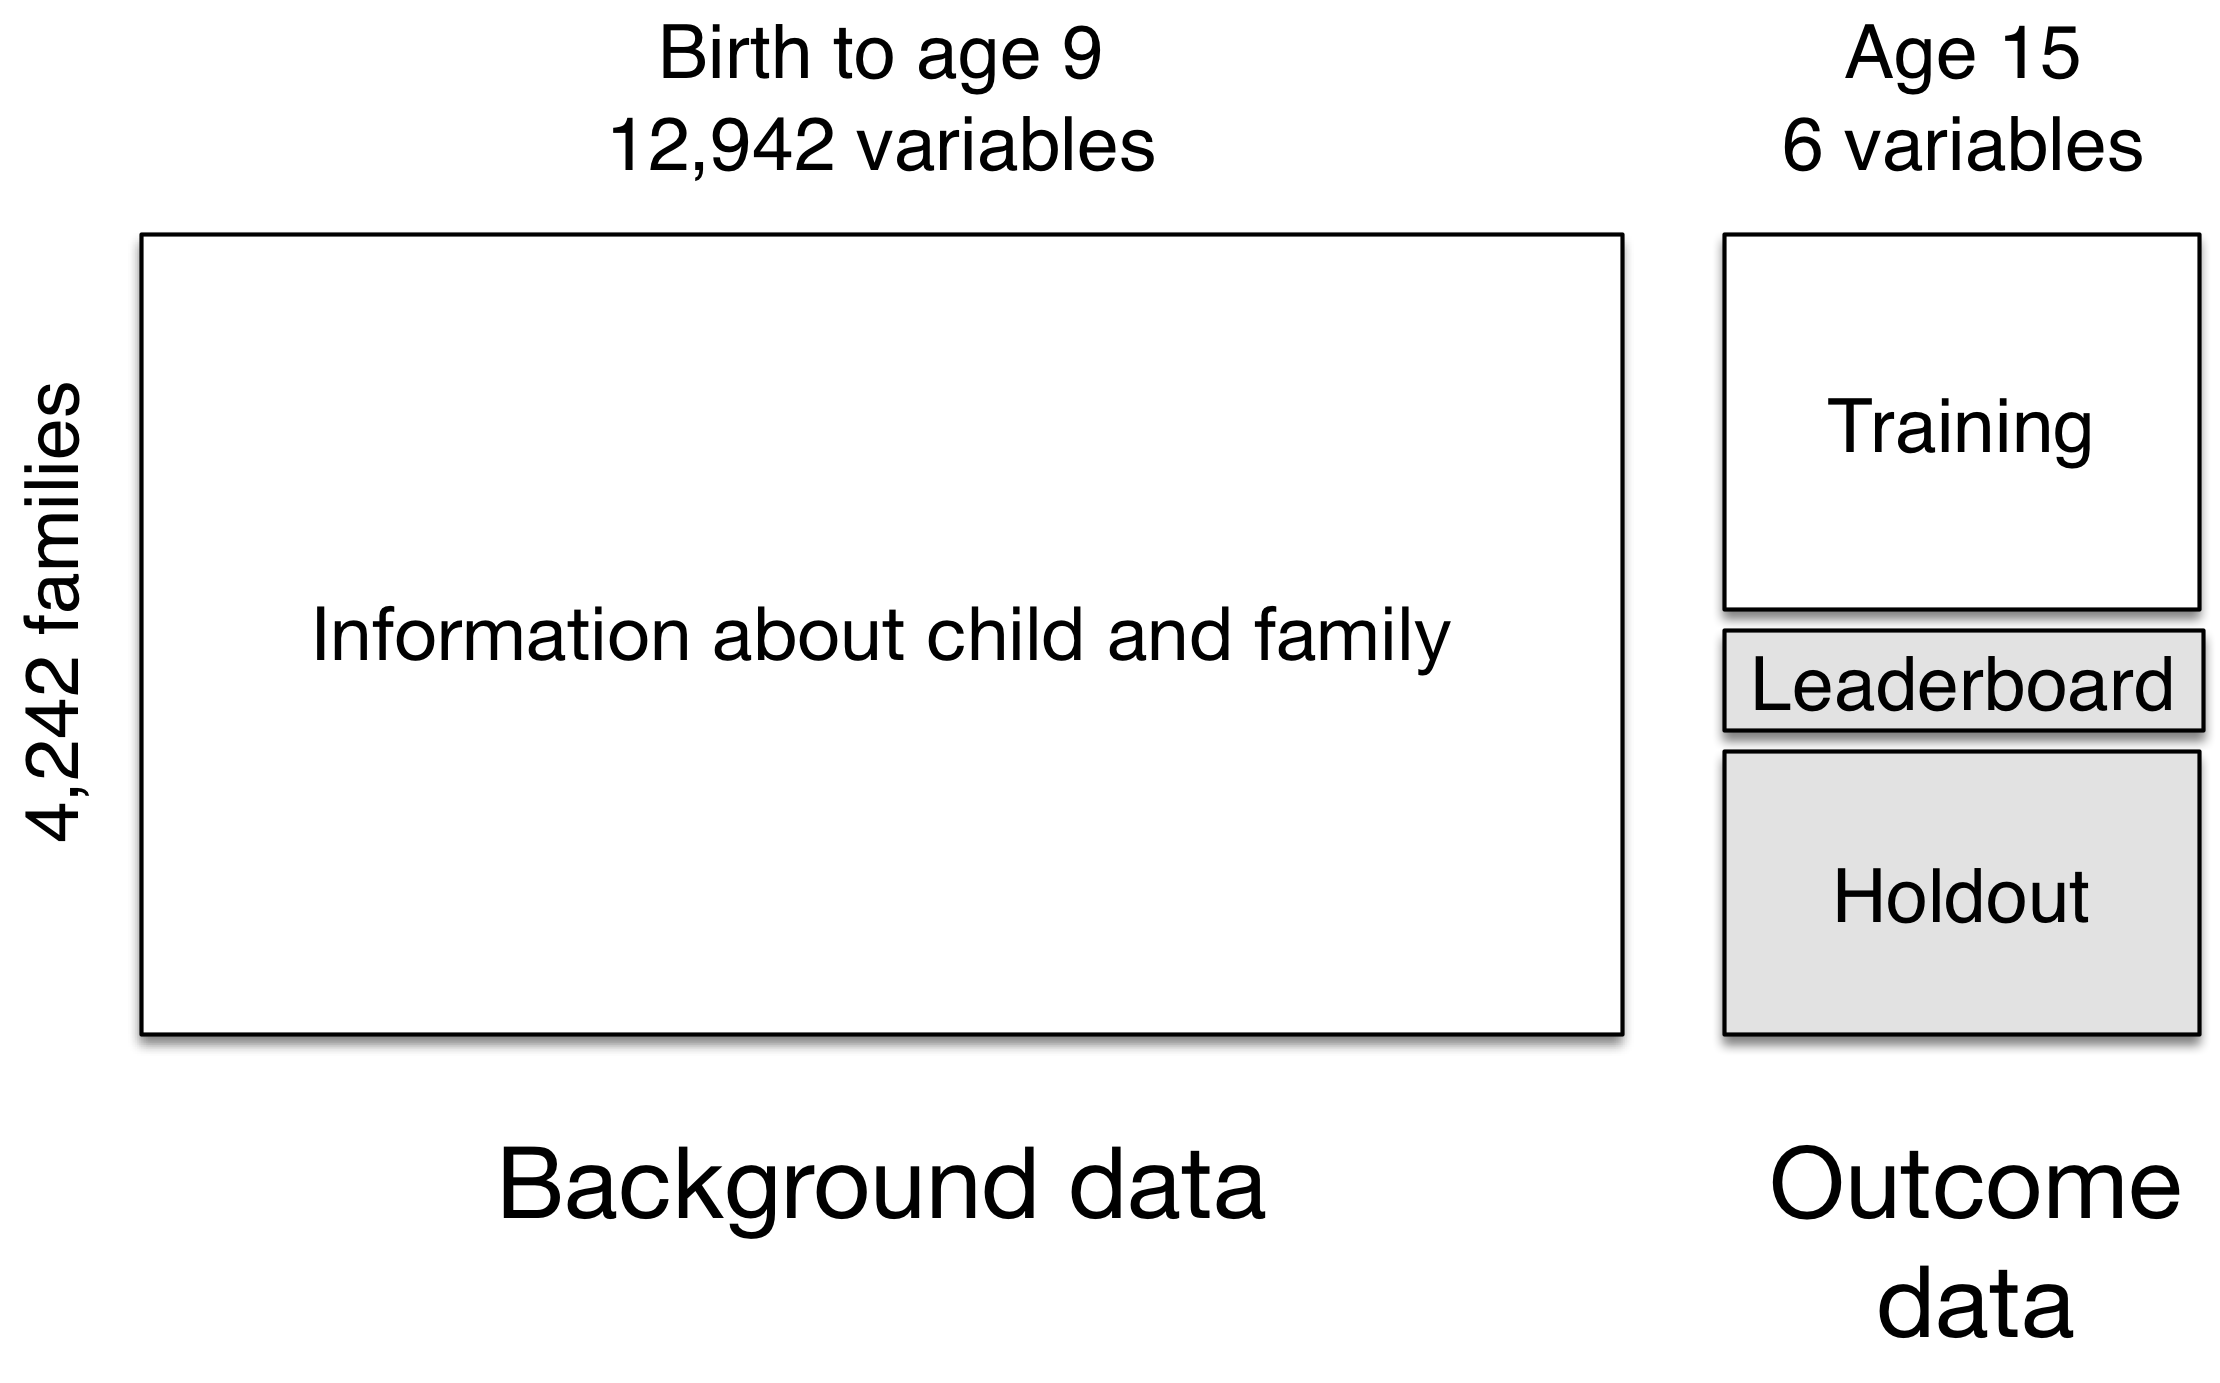
\includegraphics[width=\textwidth]{figures/ffc_design_matrix_ml}
\end{center}

\end{frame}
%%%%%%%%%%%%%%%%%%%%%%%%%
\begin{frame}

Outcomes
\begin{itemize}
\item Child: GPA (continuous), Grit (continuous)
\item Household:  Eviction (binary), Material hardship (continuous)
\item Primary care giver: Job training (binary), Job loss (binary)
\end{itemize}

\end{frame}
%%%%%%%%%%%%%%%%%%%%%%%%%
\begin{frame}

457 researchers applied to participate. Many worked in interdisciplinary teams. Goal: Make a prediction that minimizes mean square error on the hold-out set
\begin{equation*}
MSE_{\text{holdout}} = \frac{\sum_{i \in \text{holdout}} (\hat{y}_i - y_i)^2}{n_{holdout}}
\end{equation*}

\vfill
More on privacy and ethics audit: Lundberg et al.\ (2019)
\end{frame}
%%%%%%%%%%%%%%%%%%%%%%%%%
\begin{frame}

Using a large, high-quality social science dataset collected since birth and modern machine learning methods, how accurately can we predict outcomes from children, parents, and families?

\begin{equation*}
R^2_{holdout} = 1 - \frac{\sum_{i \in \text{holdout}} (\hat{y}_i - y_i)^2}{\sum_{i \in \text{holdout}} (\bar{y}_{train} - y_i)^2}
\end{equation*}

\pause 
\vfill

Before I show the results, let's vote . . . .

\end{frame}
%%%%%%%%%%%%%%%%%%%%%%%%%
\begin{frame}

\begin{center}
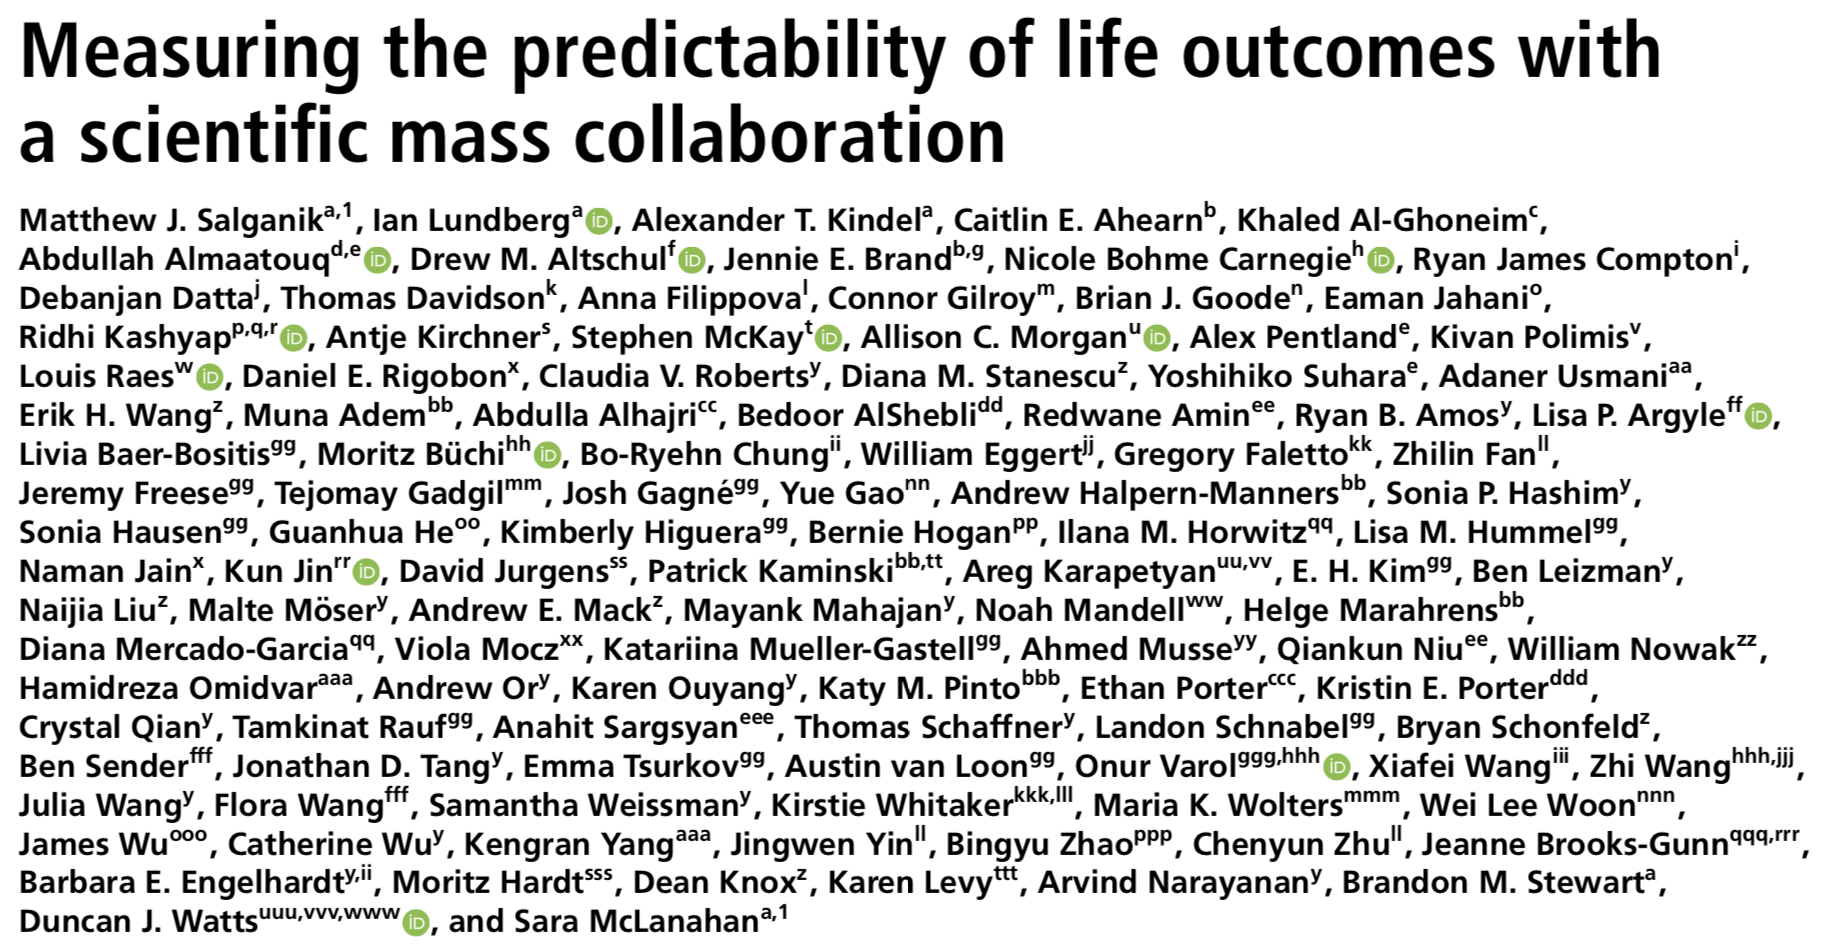
\includegraphics[width=\textwidth]{figures/salganik_measuring_2020_title_authors}
\end{center}

\end{frame}
%%%%%%%%%%%%%%%%%%%%%%%%%%

\frame{\titlepage}


\end{document}
